\documentclass[12pt, a4paper]{article}
\usepackage[utf8]{inputenc}
\usepackage[brazil]{babel}
\usepackage{graphicx}
\usepackage{amsmath}
\usepackage{amsfonts}
\usepackage{amssymb}
\usepackage{cite}
\usepackage{hyperref}
\usepackage{tikz}
\usepackage{siunitx}
\usepackage{booktabs}
\usepackage{tabularx}
\usepackage{algorithm}
\usepackage{algpseudocode}
\usepackage{float}
\usepackage{subcaption} % Para figuras compostas (se necessário)
\usepackage{float} % Para melhor posicionamento
\usetikzlibrary{shapes,arrows,positioning,calc}
\tikzstyle{startstop} = [rectangle, rounded corners, minimum width=3cm, minimum height=1cm,text centered, draw=black, fill=red!30]
\tikzstyle{io} = [trapezium, trapezium left angle=70, trapezium right angle=110, minimum width=3cm, minimum height=1cm, text centered, draw=black, fill=blue!30]
\tikzstyle{process} = [rectangle, minimum width=3cm, minimum height=1cm, text centered, draw=black, fill=orange!30]
\tikzstyle{decision} = [diamond, minimum width=3cm, minimum height=1cm, text centered, draw=black, fill=green!30]
\tikzstyle{arrow} = [thick,->,>=stealth']

\title{Plataforma Arduino: Sensores  Aplicados na Estatística}
\author{Jefferson Bezerra dos Santos}
\date{}

\begin{document}

\maketitle

\begin{abstract}
    Este artigo explora a aplicação de sensores de Arduino na coleta e análise de dados estatísticos.
    Por meio de exemplos práticos, demonstramos como essas tecnologias podem automatizar a coleta de dados e
    aprimorar análises estatísticas em tempo real. O artigo também discute limitações e aplicações futuras, com
    ênfase em IoT, aprendizado de máquina e técnicas de análise de dados e suas implementações em
    microcontroladores. Resultados mostram que a integração entre hardware acessível e métodos estatísticos
    oferecenovas oportunidades em diversas áreas como: agricultura, saúde e monitoramento ambiental.
\end{abstract}

\section{Introdução}
\label{sec:introducao}
A estatística desempenha um papel central na interpretação de dados em cenários complexos, como monitoramento ambiental
e automação industrial. Sensores baseados em Arduino, combinados com técnicas de Internet das Coisas (IoT),
permitem coletar dados em tempo real e aplicá-los a modelos estatísticos preditivos \cite{NARAYANA2024e28195}. A análise
preditiva é fundamental para compreender as relações entre diversos fatores ambientais, como temperatura, umidade e
qualidade do ar, e seu impacto na produtividade agrícola. 

Nesse contexto, a agricultura inteligente surge como um exemplo emblemático, em que sensores de baixo custo monitoram
parâmetros como umidade do solo e temperatura, gerando dados para otimização de recursos e permitindo a integração com
áreas como robótica e automação para alcançar resultados favoráveis \cite{narayan2024}. Além disso, a integração de
aprendizado de máquina com dados de sensores IoT amplia a capacidade de análise estatística, proporcionando insights
mais precisos e automatizados \cite{Adi2020}. 

O tratamento adequado dos dados e a escolha criteriosa dos métodos estatísticos são essenciais para garantir a precisão
e a eficácia das previsões. Segundo \cite{Selmy2024}, uma análise cuidadosa dos dados e dos métodos utilizados é crucial
para resultados confiáveis. Modelos tradicionais, como ARIMA e SARIMA, são eficazes em muitos cenários, mas apresentam
limitações ao lidar com dados que possuem relações não lineares e sazonalidade. Para superar essas limitações, modelos
de aprendizado profundo, como LSTM e o híbrido CNN-LSTM, têm sido empregados, demonstrando desempenho superior em
contextos específicos.

Dessa forma, o presente artigo explora a aplicação de técnicas estatísticas e sua implementação em microcontroladores da
plataforma Arduino, com foco na análise de dados em tempo real e na automação de sistemas robóticos em ambientes
dinâmicos. O estudo tem como objetivo contribuir para a otimização de processos e o aprimoramento da precisão de
previsões, destacando aplicações práticas em áreas como agricultura inteligente e sistemas Iot.

\section{Revisão da Literatura}
\label{sec:revisao}
A análise estatística de dados provenientes de sensores IoT tem ganhado relevância em aplicações industriais e
ambientais, impulsionada pela necessidade de processamento eficiente de grandes volumes de dados e pela demanda por
insights preditivos precisos. Estudos como o de \cite{Ferencz2023} demonstram o uso de técnicas estatísticas
descritivas, como regressão linear e análise de séries temporais, combinadas com métodos de aprendizado de máquina, como
\textit{Random Forest}, para o monitoramento preditivo em ambientes industriais. Essas abordagens têm se mostrado
eficazes na identificação de padrões complexos e na previsão de falhas, otimizando processos e reduzindo custos.

A rápida expansão da Internet das Coisas (IoT) e da Internet Industrial das Coisas (IIoT) tem resultado na geração
massiva de dados, o que impõe desafios significativos às indústrias, especialmente no que diz respeito ao processamento
em tempo real. Algoritmos tradicionais frequentemente apresentam limitações ao lidar com a complexidade e o volume
desses dados. Diante disso, \cite{Ferencz2023} propõem a utilização de técnicas robustas e inteligentes para o
tratamento preditivo de dados, destacando métodos como:

\begin{itemize}
    \item \textbf{Regressão Linear}: Técnica que analisa a relação entre variáveis, permitindo prever valores dependentes com base em variáveis independentes.
    \item \textbf{Random Forest}: Modelo de aprendizado de máquina baseado em múltiplas árvores de decisão, que aumenta a precisão das previsões e é eficaz na identificação de padrões complexos.
    \item \textbf{Detecção de Outliers}: Conjunto de técnicas utilizadas para identificar e tratar dados que se desviam significativamente do padrão esperado, melhorando a qualidade da análise.
    \item \textbf{Análise de Séries Temporais}: Métodos aplicados à análise de dados ao longo do tempo, permitindo identificar tendências, ciclos e padrões para embasar decisões operacionais e de manutenção.
\end{itemize}

De forma complementar, \cite{Syafrudin2018} aplicam técnicas de \textit{machine learning} para monitorar processos de
manufatura em tempo real. O estudo propõe um sistema de monitoramento baseado em sensores IoT, processamento de grandes
volumes de dados (\textit{big data}) e um modelo de predição híbrido, que combina DBSCAN para detecção de outliers e
\textit{Random Forest} para classificação de falhas. Esse sistema foi implementado em uma linha de montagem automotiva
na Coreia, demonstrando eficácia na prevenção de perdas e na melhoria da tomada de decisão. Para o processamento de
dados, foram utilizadas ferramentas como Apache Kafka, Apache Storm e MongoDB, que garantem escalabilidade e eficiência
no tratamento de grandes volumes de informações.

No contexto agrícola, \cite{narayan2024} revisam sistemas IoT que utilizam microcontroladores Arduino para coleta de
dados, destacando a importância de métodos estatísticos robustos. A pesquisa evidencia o impacto transformador da IoT na
agricultura inteligente, com a integração de sensores e microcontroladores permitindo o monitoramento em tempo real de
condições ambientais e a otimização de práticas agrícolas. Foram explorados protocolos de comunicação como LoRa, ZigBee
e WiFi, que garantem a transmissão eficaz de dados mesmo em áreas rurais com conectividade limitada. Entre os benefícios
destacados estão a economia de água e insumos, além da promoção de práticas mais sustentáveis. No entanto, os autores
também apontam desafios, como os altos custos de implementação e a necessidade de garantir segurança e privacidade dos
dados coletados. A colaboração entre setores como tecnologia da informação, ciência ambiental e políticas públicas é
apontada como essencial para superar essas barreiras e facilitar a adoção em larga escala da IoT na agricultura.

Em 2023, \cite{pica2023} analisaram a penetração de dispositivos IoT em residências na União Europeia, destacando o
aumento do uso desses dispositivos entre 2020 e 2022. O estudo, baseado em dados do Eurostat, identifica que os
principais fatores que dificultam a adoção da IoT são a "falta de necessidade" e o "custo dos dispositivos", cuja
influência diminuiu ao longo do tempo. Os resultados evidenciam diferenças significativas na adoção de IoT entre os
Estados-Membros, sugerindo a necessidade de estratégias e políticas públicas direcionadas para estimular a adoção em
categorias específicas e promover as vantagens econômicas e de eficiência que a tecnologia pode oferecer.

No campo da análise preditiva, \cite{Selmy2024} propõem uma nova estrutura focada na previsão de séries temporais,
especialmente de temperatura, utilizando dados de sensores IoT. O estudo compara modelos tradicionais, como ARIMA e
SARIMA, com abordagens baseadas em aprendizado profundo, como LSTM e um modelo híbrido CNN-LSTM. Os resultados
demonstram que os modelos de aprendizado profundo, em especial o CNN-LSTM, apresentam desempenho superior, com redução
significativa nas taxas de erro e maior capacidade de capturar sazonalidade e tendências nas séries temporais. Para o
processamento de dados, foram utilizadas tecnologias de código aberto, como Apache Spark e Kafka, que garantem
escalabilidade e eficiência. No entanto, o estudo também enfrentou desafios, como a complexidade dos dados provenientes
de múltiplos sensores e a demanda por recursos computacionais significativos para o ajuste e validação dos modelos.

Por fim, \cite{NARAYANA2024e28195} apresentam um sistema inovador de monitoramento ambiental em tempo real baseado em
IoT, que utiliza uma rede diversificada de sensores para coletar dados sobre parâmetros como qualidade do ar,
temperatura, umidade, pH da água e turbidez. Entre os sensores utilizados, destacam-se:

\begin{itemize}
    \item \textbf{Sensor de Temperatura e Umidade (DHT11)}: Fornece dados precisos para identificar mudanças climáticas e condições ambientais.
    \item \textbf{Sensores de Velocidade e Direção do Vento}: Monitoram condições do vento, importantes para a previsão de incêndios florestais.
    \item \textbf{Sensores de Precipitação}: Incluem pluviómetros e sensores de gotas de chuva, vitais para prever inundações e monitorar níveis hídricos.
\end{itemize}

A integração desses sensores em um sistema IoT permite acesso remoto e em tempo real aos dados, além de fomentar a
conscientização pública sobre questões ambientais. No entanto, o sistema enfrenta desafios relacionados à conectividade,
segurança, privacidade e escalabilidade, que precisam ser superados para garantir sua eficácia em diferentes contextos.


\section{Metodologia}
\label{sec:metodologia}

Nessa secção é apresentada metodologia para a integração de sensores com a plataforma Arduino, aplicando
técnicas estatísticas e matemáticas para análise de dados. A abordagem é voltada para aplicações práticas, com
embasamento teórico robusto, visando a coleta, processamento e análise de dados de forma criteriosa. A metodologia é
dividida nas seguintes etapas:

\subsection{Definição do Problema}
\subsubsection{Objetivos}
O objetivo principal é explorar a utilização de sensores em conjunto com técnicas estatísticas e matemáticas
para aplicações em cenários práticos, como monitoramento ambiental, automação residencial ou controle de processos
envolvendo IoT. Os objetivos específicos incluem:
\subsubsection{Os objetivos específicos}
Os objetivos específicos incluem:

\begin{itemize}
    \item Coletar dados de variáveis físicas (temperatura, umidade, qualidade do ar, etc.) por meio de sensores conectados à plataforma Arduino.
    \item Aplicar técnicas estatísticas descritivas e inferenciais para análise dos dados.
    \item Utilizar modelos matemáticos e estátisticos para previsão e tomada de decisão.
    \item Integrar o Arduino com Python para comunicação e controle de sensores com base nos resultados das análises.
    \item Validar a eficácia do sistema em cenários práticos, com embasamento matemático e estatístico.
\end{itemize}

\subsection{Materiais e Equipamentos}
Para a execução do projeto, foram utilizados os seguintes materiais e equipamentos:
\begin{itemize}
    \item \textbf{Plataforma Arduino}: Microcontrolador Arduino Uno ou similar.
    \item \textbf{Sensores}: DHT11 (temperatura e umidade do ar) e HD-38 (umidade do solo).
    \item \textbf{Componentes eletrônicos}: Resistores, jumpers, protoboard,  módulo sdcard.
    \item \textbf{Software}:
        \begin{itemize}
            \item \textbf{Arduino-cli}: Para programação do microcontrolador e automação.
            \item \textbf{Python}: Para análise de dados e estatística.
            \item \textbf{Bibliotecas Python}: Pandas, NumPy, Matplotlib, Seaborn, Scikit-learn, TensorFlow, PySerial.
        \end{itemize}
\end{itemize}

\subsection{Arquitetura do Sistema}
\label{sec:implementacao}

O sistema foi implementado utilizando uma placa Arduino com sensor DHT11 para coleta de dados de temperatura e umidade do ar conjuntamente com um sensor HD-38 de umidade do solo. A Figura~\ref{fig:diagrama_blocos} apresenta a arquitetura geral do sistema.


\begin{figure}[h]
    \centering
    \begin{tikzpicture}[node distance=1.8cm, auto, >=stealth']
        % Blocos
        \node (inicio) [startstop] {Início};
        \node (init) [process, below of=inicio] {Inicialização do Sistema};
        \node (sensor) [io, below of=init] {Sensores};
        \node (arduino) [process, below of=sensor] {Processamento Arduino};
        \node (serial) [io, below of=arduino] {Saída};
        \node (fim) [startstop, below of=serial] {Loop Contínuo};

        % Linhas
        \draw [->] (inicio) -- (init);
        \draw [->] (init) -- (sensor);
        \draw [->] (sensor) -- (arduino);
        \draw [->] (arduino) -- (serial);
        \draw [->] (serial) -- (fim);
        \draw [->] (fim.east) -- ++(1.5,0) |- node[near start,right] {} (sensor.east);

        % Legenda
        \node at (8,-3) [text width=4cm] {
            \scriptsize
            \begin{description}
                \item[Início/Parada:] Operações de inicialização
                \item[Processo:] Transformação de dados
                \item[Entrada/Saída:] Interface com componentes
            \end{description}
        };
    \end{tikzpicture}
    \caption{Diagrama de blocos do sistema de aquisição de dados}
    \label{fig:diagrama_blocos}
\end{figure}

O diagrama de blocos apresenta a cadeia operacional do sistema, compreendendo: (1) ativação dos sensores  para captura
de dados ambientais, (2) condicionamento do sinal pela plataforma Arduino, e (3) transmissão dos parâmetros processados
via comunicação serial para monitoramento e escrita em arquivo para processamento dos dados. Na sequência, apresenta-se a estrutura lógica do algoritmo desenvolvido para
coleta e processamento dos dados.

\subsection{Fluxo de Controle}
Apresenta-se abaixo o diagrama de fluxo de controle do sistema, que descreve graficamente o algoritmo de aquisição e processamento dos dados ambientais.

\begin{figure}[!ht]
    \centering
    \begin{tikzpicture}[
            node distance=1.0cm,
            box/.style={draw, rectangle, rounded corners, minimum width=2.5cm, minimum height=1cm, text centered, align=center, fill=blue!30, thick},
            decision/.style={draw, diamond, aspect=2, minimum width=2.5cm, minimum height=1cm, text centered, align=center, fill=yellow!30, thick},
            cloud/.style={draw, ellipse, minimum height=1cm, minimum width=2cm, fill=red!30, thick},
            arrow/.style={->, >=stealth', shorten >=1pt, thick},
            titlebox/.style={draw, rectangle, fill=black!10, inner sep=5pt, rounded corners}
            ]

            % Caixa de contorno principal
            \begin{scope}[on background layer]
                \node [draw, rectangle, rounded corners, fill=gray!5, thick, inner sep=0.5cm, fit=(inicio) (armazenamento) (erro) (correlacao)] (box) {};
            \end{scope}

            % Nós do diagrama
            \node (inicio) [box] {Inicialização};
            \node (leitura) [box, below=of inicio] {Leitura do Sensor};
            \node (validacao) [decision, below=of leitura] {Valores\\Válidos?};
            \node (armazenar) [box, below right=1cm and 1cm of validacao] {Armazenar\\em Buffers};
            \node (erro) [cloud, below left=1cm and 1cm of validacao] {Log\\de Erro};
            \node (estatisticas) [box, below=of armazenar] {Calcular\\Estatísticas};
            \node (correlacao) [box, right=of estatisticas] {Atualizar\\Correlação};
            \node (outliers) [box, below=of estatisticas] {Detectar\\Outliers};
            \node (significancia) [box, below=of correlacao] {Testar\\Significância};
            \node (armazenamento) [box, below=of $(outliers.south)!0.5!(significancia.south)$] {Armazenar\\Dados};

            % Conexões
            \draw [arrow] (inicio) -- (leitura);
            \draw [arrow] (leitura) -- (validacao);
            \draw [arrow] (validacao) -| node[above left] {Não} (erro);
            \draw [arrow] (validacao) -| node[above right] {Sim} (armazenar);
            \draw [arrow] (armazenar) -- (estatisticas);
            \draw [arrow] (armazenar) -- (correlacao);
            \draw [arrow] (estatisticas) -- (outliers);
            \draw [arrow] (correlacao) -- (significancia);
            \draw [arrow] (outliers) -- (armazenamento);
            \draw [arrow] (significancia) -- (armazenamento);

            % Título dentro da caixa
            %\node (titulo) [titlebox, above=0.3cm of inicio, font=\large\bfseries] {Fluxograma do Sistema de Monitoramento Estatístico};

            % Legenda
            \node [above=0.2cm of validacao, font=\footnotesize\itshape] {Nó de Decisão};
            \node [above=0.2cm of erro, font=\footnotesize\itshape] {Tratamento de Exceção};

            % Grade de referência (opcional - comentar na versão final)
            %\draw [help lines] (-5,-10) grid (5,2);
    \end{tikzpicture}
    \caption{Fluxograma do processo de análise estatística com tratamento de erros e validação de dados}
    \label{fig:fluxograma_estatistico}
\end{figure}

Conforme ilustrado na Figura~\ref{fig:fluxograma_estatistico}, o processo de aquisição de dados inicia-se com a coleta simultânea
dos parâmetros de temperatura e umidade relativa do ar. Esses dados brutos são então submetidos a uma estrutura de
controle de qualidade, onde sua validade é verificada. Após a validação bem-sucedida, o algoritmo prossegue com o fluxo
padrão de processamento e transmissão dos dados

\subsection{Coleta de Dados}
A coleta de dados será realizada por meio de sensores conectados à plataforma Arduino, seguindo as seguintes etapas:
\begin{itemize}
    \item \textbf{Configuração dos Sensores}: Montagem do circuito e calibração dos sensores.
    \item \textbf{Programação do Arduino}: Desenvolvimento de código para leitura dos dados em intervalos de tempo definidos.
    \item \textbf{Comunicação com Python}: Utilização da biblioteca \textbf{PySerial} para estabelecer comunicação serial entre o Arduino e o Python, permitindo a transmissão dos dados coletados para o ambiente Python em tempo real.
    \item \textbf{Armazenamento dos Dados}: Os dados foram  armazenados localmente em arquivos CSV.
\end{itemize}

\subsection{Análise Estatística }
Os dados coletados foram processados e analisados utilizando Python e suas bibliotecas, com embasamento matemático e
estatístico detalhado:

\subsubsection{Processamento}
Um \textbf{outlier} é uma observação atípica que se distância significativamente das demais amostras em um conjunto de dados. Formalmente, para uma variável aleatória $X$, um valor $x_i$ é considerado outlier se:

\begin{itemize}
        \begin{equation}
            \text{Outlier} = \begin{cases}
                x_i < Q1 - k \cdot IQR \\
                x_i > Q3 + k \cdot IQR
            \end{cases}
        \end{equation}
\end{itemize}

onde:

\begin{itemize}
    \item $Q_1$ é o primeiro quartil (percentil 25)
    \item $Q_3$ é o terceiro quartil (percentil 75)
    \item $\text{IQR} = Q_3 - Q_1$ é o intervalo interquartil
    \item $k$ é uma constante (tipicamente 1.5 para outliers moderados ou 3.0 para outliers extremos)
\end{itemize}

Sua utilização torna o sistema mais robusto, uma vez que valores discrepantes (outliers) podem
surgir devido a erros de medição dos sensores causados por problemas de hardware. Dessa forma, a
remoção, correção ou tratamento desses outliers garante que a análise estatística seja realizada sem
a influência de dados distorcidos. 


\subsubsection{Medidas de Tendência Central}
Para um conjunto de dados $\{x_1, x_2, \dots, x_n\}$ amostrados pelo sensor, definimos:

\begin{itemize}
    \item \textbf{Média aritmética}:
        \begin{equation}
            \bar{x} = \frac{1}{n}\sum_{i=1}^n x_i
        \end{equation}

    \item \textbf{Mediana}:
        \begin{equation}
            Q_2 = \begin{cases}
                x_{\left(\frac{n+1}{2}\right)} & \text{se } n \text{ ímpar}\\
                \frac{x_{\left(\frac{n}{2}\right)} + x_{\left(\frac{n}{2}+1\right)}}{2} & \text{se } n \text{ par}
            \end{cases}
        \end{equation}
\end{itemize}

\subsubsection{Medidas de Dispersão}
A variabilidade dos dados é quantificada por:

\begin{itemize}
    \item \textbf{Variância}:
        \begin{equation}
            {\sigma}^2 = \frac{1}{n-1}\sum_{i=1}^n (x_i - \bar{x})^2
        \end{equation}

    \item \textbf{Desvio padrão}:
        \begin{equation}
            {\sigma} = \sqrt{{\sigma}^2}
        \end{equation}

    \item \textbf{Intervalo Interquartil (IQR)}:
        \begin{equation}
            \text{IQR} = Q_3 - Q_1
        \end{equation}
\end{itemize}

\subsubsection{Justificativa para o Projeto}
A análise descritiva é fundamental porque:

\begin{enumerate}
    \item A \textbf{comparação média-mediana} identifica assimetrias:
        \begin{equation}
            \Delta = |\bar{x} - Q_2|
        \end{equation}
        Valores $\Delta > 0.1s$ indicam presença de outliers.

    \item O \textbf{desvio padrão} $s$ quantifica a precisão do sensor:
        \begin{equation}
            \text{Precisão} \propto \frac{1}{s}
        \end{equation}

    \item O \textbf{IQR} define limites operacionais robustos:
        \begin{equation}
            \text{Limites} = \left[ Q_1 - 1.5 \times \text{IQR}, Q_3 + 1.5 \times \text{IQR} \right]
        \end{equation}

        essenciais para detecção de falhas.
\end{enumerate}

\begin{table}[h]
    \centering
    \caption{Métricas utilizadas em sensores IoT}
    \label{tab:metricas_iot}
    \begin{tabular}{|p{4cm}|p{8cm}|}
        \toprule
        \textbf{Métrica} & \textbf{Relevância} \\
        \hline
        Média & Utilizada para o monitoramento contínuo dos dados coletados pelos sensores. \\
        \hline
        Mediana & Aplicada no controle dos sensores, reduzindo o impacto de valores atípicos. \\
        \hline
        IQR (Intervalo Interquartil) & Empregado na detecção de anomalias, identificando variações inesperadas nos dados. \\
        \hline
        Desvio padrão ($s$) & Essencial para a calibração do sensor, permitindo avaliar a dispersão dos valores medidos. \\
        \bottomrule
    \end{tabular}
    \legend{Fonte: Elaborado pelo autor.}
\end{table}


\subsection{Análise de Correlação Linear para Sistemas Embarcados}
\label{subsec:correlacao}

A análise de dependência estocástica entre as variáveis ambientais coletadas (temperatura $T$ e umidade relativa $U$) foi realizada mediante o coeficiente de correlação momento-produto de Pearson, cuja forma populacional é dada por:

\begin{equation}
    \rho_{TU} = \frac{\mathbb{E}[(T - \mu_T)(U - \mu_U)]}{\sigma_T \sigma_U} = \frac{\text{Cov}(T,U)}{\sqrt{\text{Var}(T)\text{Var}(U)}}
\end{equation}

\noindent Para amostras finitas, utilizamos o estimador não-tendencioso:

\begin{equation}
    r_{TU} = \frac{\sum_{i=1}^n (T_i - \bar{T})(U_i - \bar{U})}{\sqrt{\sum_{i=1}^n (T_i - \bar{T})^2 \sum_{i=1}^n (U_i - \bar{U})^2}}
    \label{eq:pearson_amostral}
\end{equation}

\subsubsection{Justificativa Matemática para Implementação em Arduino}
\begin{itemize}
    \item \textbf{Eficiência Computacional}: A equação (\ref{eq:pearson_amostral}) requer apenas:
        \begin{itemize}
            \item $4n$ operações de soma
            \item $2n$ multiplicações
            \item 1 divisão e 1 raiz quadrada
        \end{itemize}
    \item \textbf{Otimização de Memória}: Pode ser calculada em streaming, armazenando apenas:
        \begin{equation}
            S_T = \sum T_i,\; S_U = \sum U_i,\; S_{TU} = \sum T_iU_i,\; S_{T^2} = \sum T_i^2,\; S_{U^2} = \sum U_i^2
        \end{equation}
    \item \textbf{Precisão Numérica}: A fórmula é numericamente estável para valores típicos de sensores ($-40°C \leq T \leq 125°C$, $0\% \leq U \leq 100\%$)
\end{itemize}

\subsubsection{Teste de Hipótese com Restrições Computacionais}
Para verificação da significância estatística em sistemas embarcados, utilizamos a transformação de Fisher com aproximação para pequenas amostras:

\begin{equation}
    z = \frac{1}{2}\ln\left(\frac{1+r}{1-r}\right) \sim \mathcal{N}\left(\frac{1}{2}\ln\left(\frac{1+\rho}{1-\rho}\right), \frac{1}{\sqrt{n-3}}\right)
    \label{eq:fisher}
\end{equation}

\noindent Permitindo calcular intervalos de confiança assintóticos mesmo com $n < 30$.

\subsubsection{Interpretação Físico-Estatística para Sensores IoT}
\begin{table}[h]
    \centering
    \caption{Interpretação de Correlações em Ambientes Controlados}
    \begin{tabularx}{\linewidth}{|l|X|X|}
        \toprule
        \textbf{$\rho$} & \textbf{Interpretação Física} & \textbf{Ação no Arduino} \\
        \midrule
        $0.9 \leq \rho \leq 1$ & Acoplamento termodinâmico perfeito & Reduzir taxa de amostragem em 50\% \\
        \hline
        $-0.9 \leq \rho \leq -0.7$ & Resfriamento evaporativo ativo & Ativar ventilação forçada \\
        \hline
        $|\rho| < 0.2$ & Falha de sensor ou ambiente anômalo & Acionar diagnóstico de hardware \\
        \bottomrule
    \end{tabularx}
\end{table}

\subsubsection{Implementação Otimizada}
O algoritmo no Arduino segue:

\begin{enumerate}
    \item Amostragem em janelas móveis de $n=30$ pontos (balanceando precisão e latência)
    \item Cálculo recursivo das somas acumuladas
    \item Atualização da correlação a cada 5 novas amostras
    \item Limiarização adaptativa baseada em histórico
\end{enumerate}

\begin{algorithm}[H]
    \caption{Cálculo Recursivo de $\rho$ para Arduino}
    \begin{algorithmic}[1]
        \State Inicializar $S_T, S_U, S_{TU}, S_{T^2}, S_{U^2} \gets 0$
        \For{cada nova amostra $(T_i, U_i)$}
        \State Atualizar somas acumuladas
        \If{$i \mod 5 = 0$}
        \State Calcular $r \gets \frac{nS_{TU} - S_TS_U}{\sqrt{(nS_{T^2}-S_T^2)(nS_{U^2}-S_U^2)}}$
        \State Testar $H_0: \rho = 0$ via equação (\ref{eq:fisher}).
        \EndIf
        \EndFor
    \end{algorithmic}
\end{algorithm}


\subsection{Validação e Testes}
Para garantir a confiabilidade do sistema, serão realizados testes e validações:
\begin{itemize}
    \item \textbf{Testes de Consistência}: Repetição das medições para verificar a precisão dos sensores.
    \item \textbf{Ajustes no Modelo}: Refinamento dos algoritmos estatísticos e de aprendizado de máquina com base no desempenho observado.
    \item \textbf{Testes em Cenários Reais}: Implementação do sistema em ambientes controlados (ex.: estufa agrícola, linha de produção industrial) para avaliar sua eficácia prática.
\end{itemize}

\subsection{Implementação do Sistema de Coleta de Dados}
\label{sec:implementacao}

O sistema de coleta e análise de dados foi implementado em uma arquitetura embarcada composta por um microcontrolador Arduino Nano integrado a sensores ambientais e um módulo de armazenamento. 

\subsubsection{Arquitetura do Sistema}
O sistema possui três componentes principais:

\begin{itemize}
    \item \textbf{Camada de Aquisição}: Sensor DHT11 para medição contínua de temperatura ($T$) e umidade relativa do ar ($U_{ar}$). Sensor HD-38 para medição contínua da umidade do solo ($U_s$). 
    \item \textbf{Camada de Processamento}: Microcontrolador ATmega328P com algoritmo estatístico implementado.
    \item \textbf{Camada de Armazenamento}: Módulo SD Card para registro persistente dos dados.
\end{itemize}

\subsubsection{Algoritmo de Coleta e Processamento}
O processo de coleta segue um pipeline estatístico em tempo real:

\begin{enumerate}
    \item \textbf{Amostragem}: Leituras periódicas com intervalo $\Delta t = 5$ min.
    \item \textbf{Pré-processamento}: Validação de dados através da função:

        \begin{equation}
            \text{valid}(T,U) = 
            \begin{cases}
                1 & \text{se } T \in [-40,125] \SI{}{\celsius} \; \text{e} \; U \in [0,100]\% \\
                0 & \text{caso contrário}
            \end{cases}
        \end{equation}

    \item \textbf{Buffer Circular}: Armazenamento das últimas $N=12$ amostras para cálculo das estatísticas descritivas.
\end{enumerate}

\subsubsection{Análise Estatística Implementada}
O sistema calcula em tempo real:

\begin{itemize}
    \item \textbf{Estatísticas Descritivas}:
        \begin{itemize}
            \item Média;
            \item Mediana;
            \item Desvio-padrão;
            \item Variância.
        \end{itemize}

    \item \textbf{Detecção de Outliers}
        \begin{itemize}
            \item Método IQR.
        \end{itemize} 

\end{itemize}

\subsubsection{Armazenamento de Dados}
Os dados são registrados em arquivo CSV com a seguinte estrutura:

\begin{verbatim}
Data,Hora,Temperatura,Umidade,MediaT,DesvioT,...,OutlierT,Correlacao
\end{verbatim}

A Tabela~\ref{tab:formato_dados} detalha os campos armazenados:

\begin{table}[ht]
    \centering
    \caption{Formato do arquivo de dados}
    \label{tab:formato_dados}
    \begin{tabular}{|l|l|}
        \hline
        Campo & Descrição \\ \hline
        \hline
        Data & Data da coleta (YYYY-MM-DD) \\
        \hline
        Hora & Horário da medição (HH:MM:SS) \\
        \hline
        Temperatura & Valor bruto em °C \\
        \hline
        MediaT & Média móvel ($\bar{T}$) \\
        \hline
        IQR & Intervalo interquartil \\
        \hline
        OutlierT & Indicador booleano de anomalia \\
        \hline
        Correlacao & Coeficiente $\rho_{T,U}$ de Pearson \\ \hline
    \end{tabular}
\end{table}

\subsubsection{Otimizações Implementadas}
Para operação em hardware limitado:

\begin{itemize}
    \item \textbf{Bubble Sort} otimizado para conjuntos pequenos ($n \leq 12$);
    \item Cálculo incremental de médias e variâncias;
    \item Buffer circular para economia de memória RAM;
    \item Amostragem adaptativa baseada em variação estatística.
\end{itemize}

\section{Resultados}
\label{sec:resultados}

Os dados de monitoramento ambiental coletados em 23 de abril de 2025 (13:25 às 08:00) revelaram padrões distintos nas variáveis analisadas. A Figura \ref{fig:temporal_combinado} mostra a variação conjunta das principais variáveis ao longo do período monitorado.

\subsection{Variação Temporal das Variáveis}
A seguir é feita uma análise das variáveis em relação ao tempo.

\subsubsection{Umidade do Ar}
A análise da Figura \ref{fig:temporal_umidadear} revela que a umidade do ar apresentou:
\begin{itemize}
    \item \textbf{Variação}: 85\% a 90\%
    \item \textbf{Tendência}:
    \begin{itemize}
        \item Flutuação moderada, mantendo-se majoritariamente entre 89\%-90\%;
        \item Picos máximos de 90\% em vários intervalos durante a madrugada e manhã;
        \item Reduções pontuais para 85\% associadas a variações de temperatura.
    \end{itemize}
\end{itemize}

\begin{figure}[H]
\centering
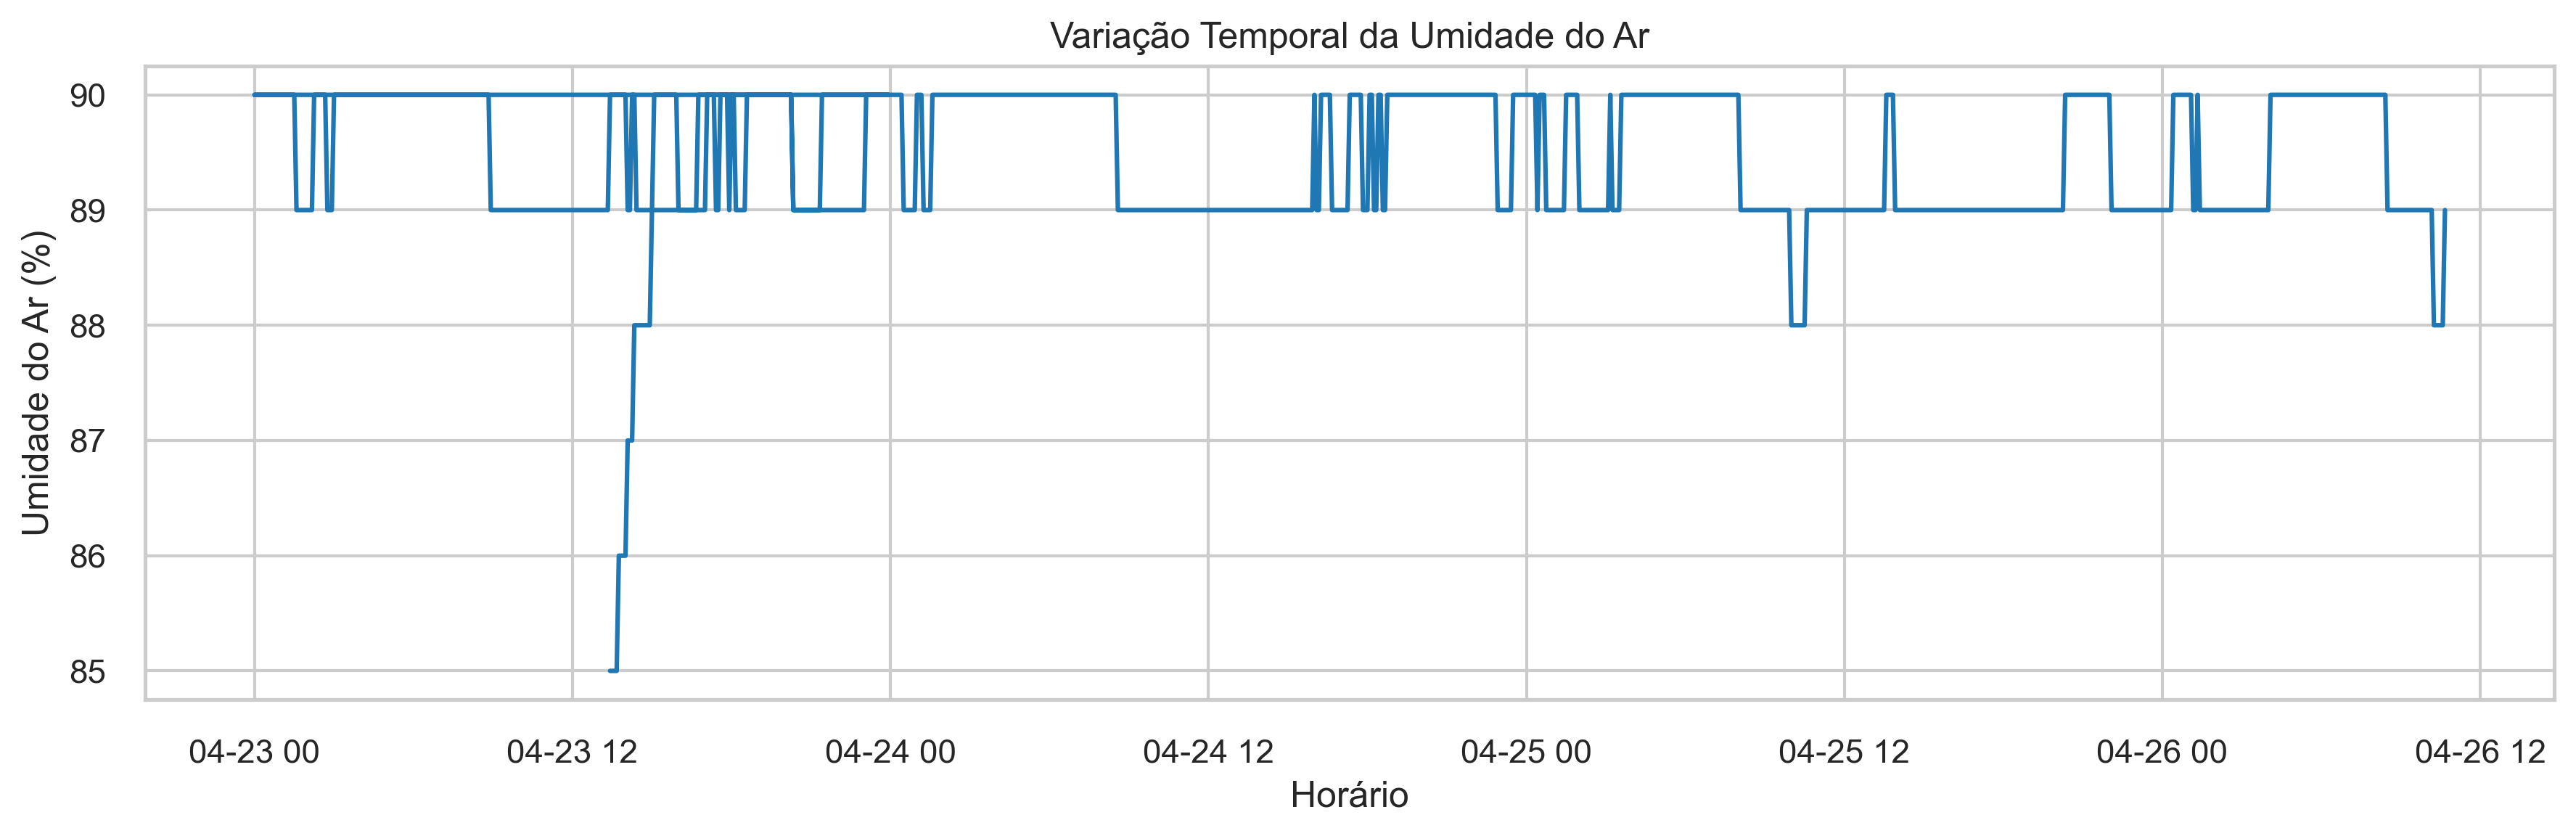
\includegraphics[width=0.9\textwidth]{graficos/temporal_umidadear.png}
\caption{Variação temporal conjunta de umidade do ar.}
\label{fig:temporal_umidadear}
\end{figure}

\subsubsection{Temperatura}
Como visível na Figura \ref{fig:temporal_temp}, a temperatura exibiu:
\begin{itemize}
    \item \textbf{Variação}: 26,9°C a 29,7°C
    \item \textbf{Tendência}:
    \begin{itemize}
        \item Elevação progressiva desde 26,9°C nas primeiras horas para 29,7°C no início da tarde;
        \item Estabilização temporária entre 28,0°C e 29,0°C durante o período noturno.
    \end{itemize}
\end{itemize}

\begin{figure}[H]
\centering
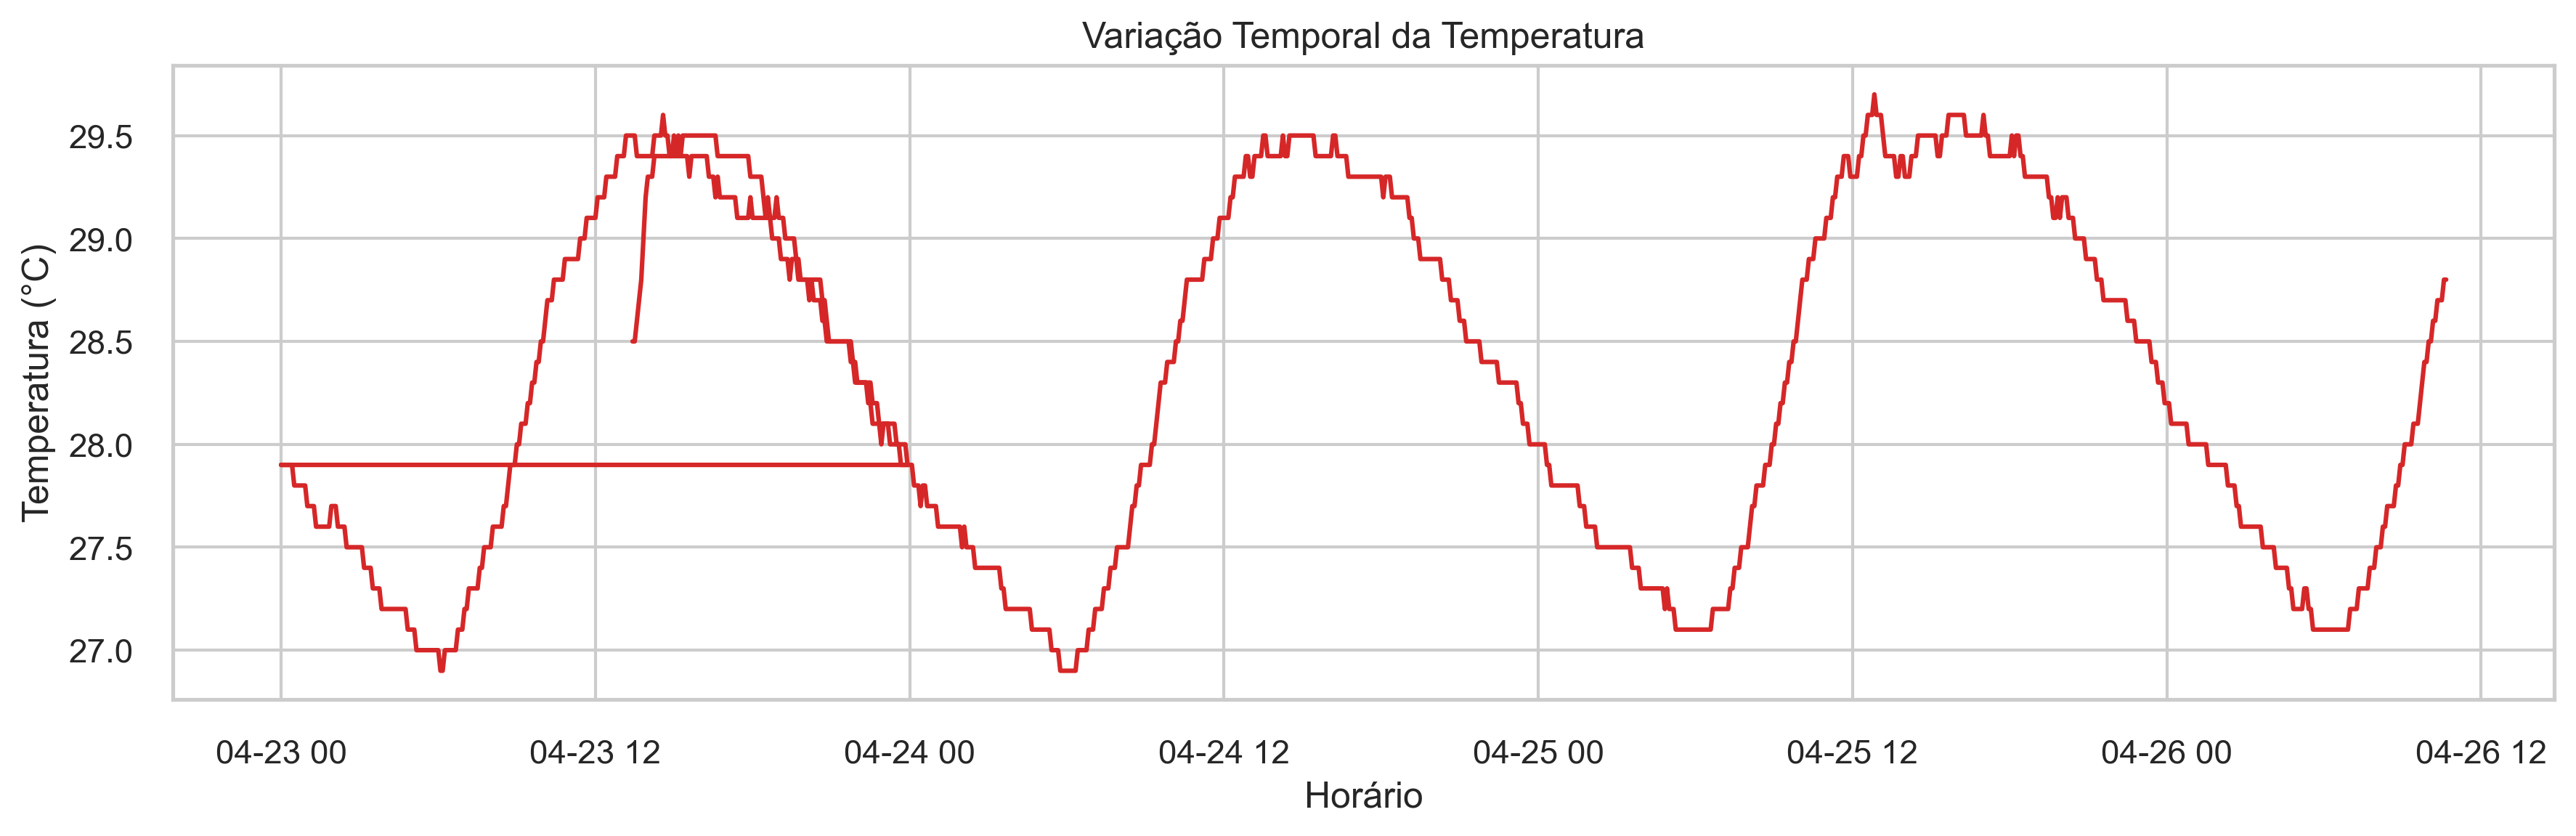
\includegraphics[width=0.9\textwidth]{graficos/temporal_temp.png}
\caption{Variação temporal da temperatura do ar.}
\label{fig:temporal_temp}
\end{figure}

\subsubsection{Umidade do Solo}
A umidade do solo apresentou uma variação mais restrita em comparação às demais variáveis ambientais. As análises revelam:

\begin{itemize}
    \item \textbf{Intervalo de variação}: 73\% a 78\%
    \item \textbf{Média}: 75{,}53\%
    \item \textbf{Desvio padrão}: 0{,}94
    \item \textbf{Mediana}: 76\%
\end{itemize}

Como ilustrado na Figura \ref{fig:boxplot}, a distribuição dos valores é relativamente concentrada, indicando baixa variabilidade. A análise de outliers baseada no intervalo interquartil (IQR) identificou alguns valores extremos próximos de 78\%, sugerindo eventos localizados de aumento da umidade do solo.

\begin{figure}[H]
\centering
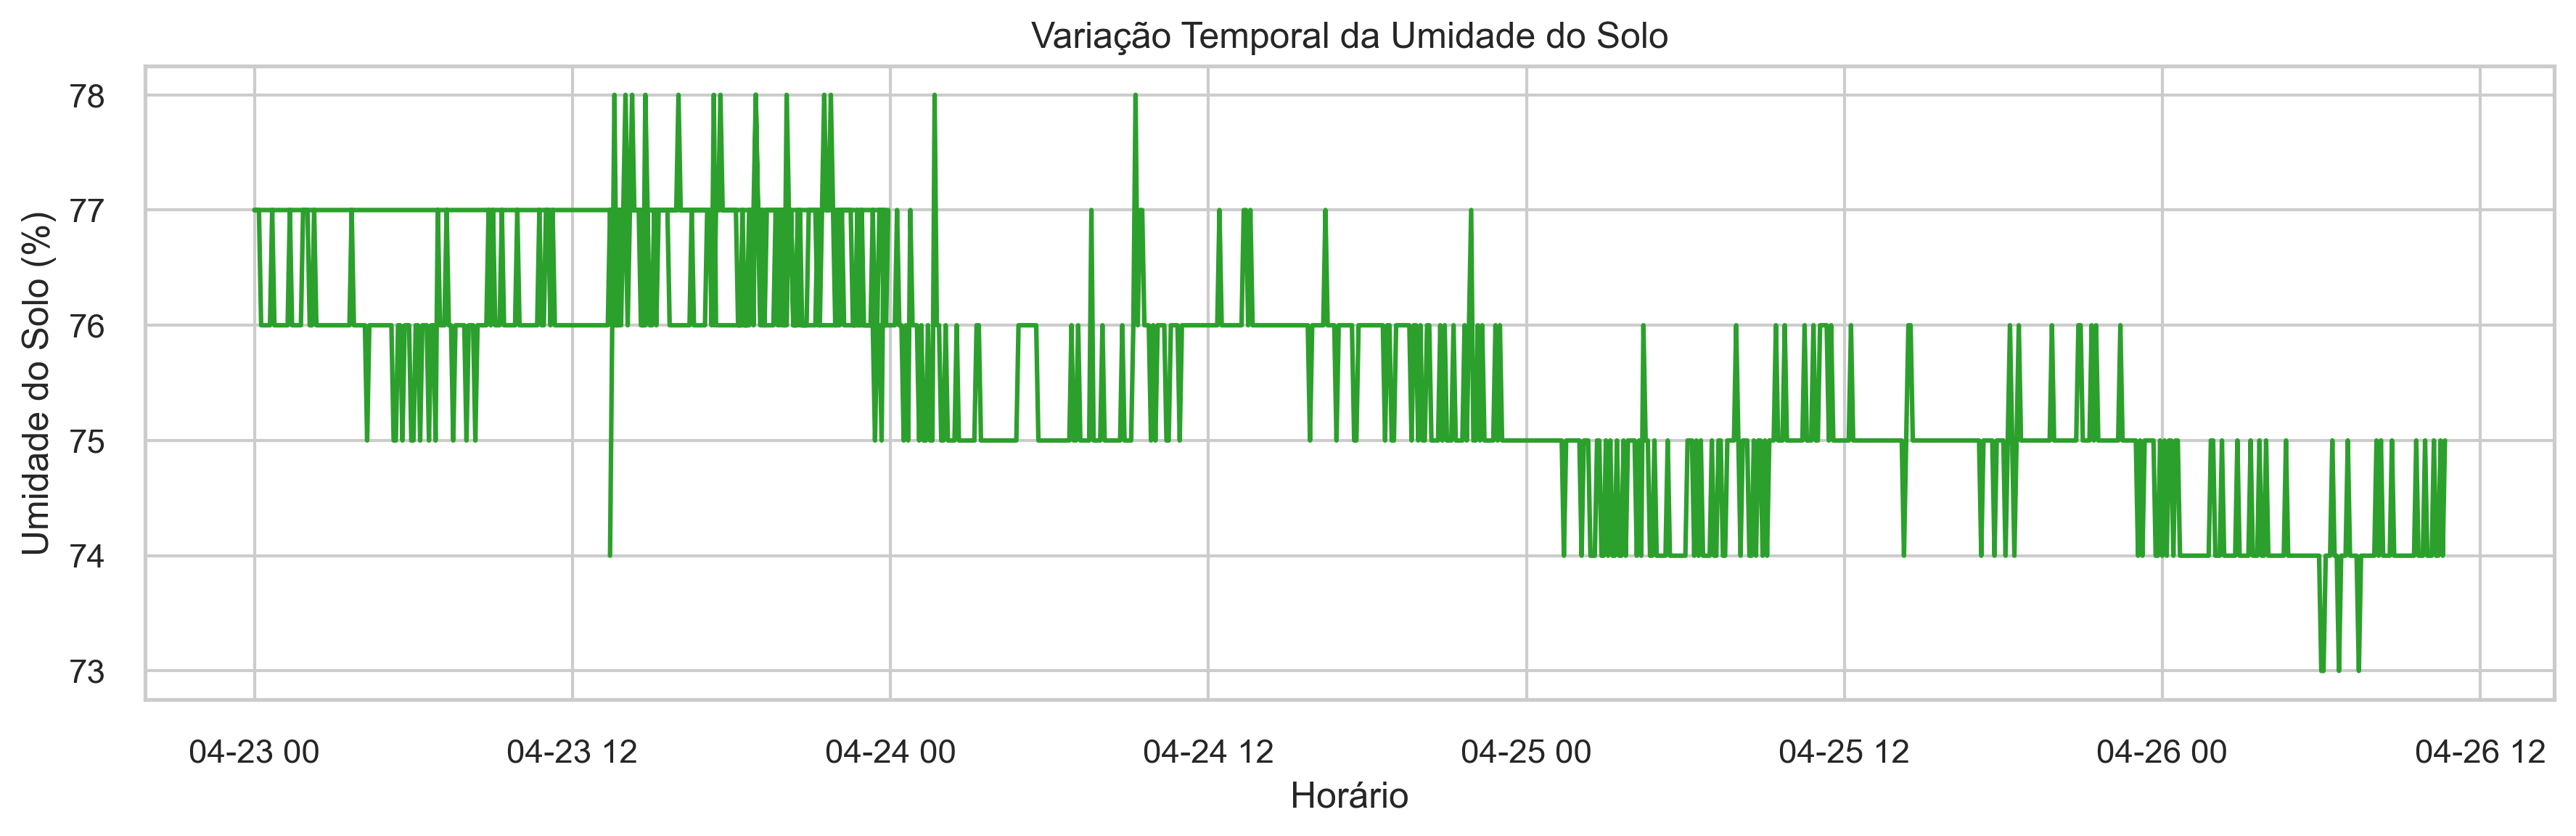
\includegraphics[width=0.9\textwidth]{graficos/temporal_usolo.png}
\caption{Variação temporal da umidade do solo.}
\label{fig:temporal_usolo}
\end{figure}

A Figura \ref{fig:temporal_combinado} apresenta a representação gráfica combinada das três variáveis monitoradas — temperatura, umidade do solo e umidade do ar — permitindo uma análise integrada de sua variação temporal ao longo do período observado.

\begin{figure}[H]
\centering
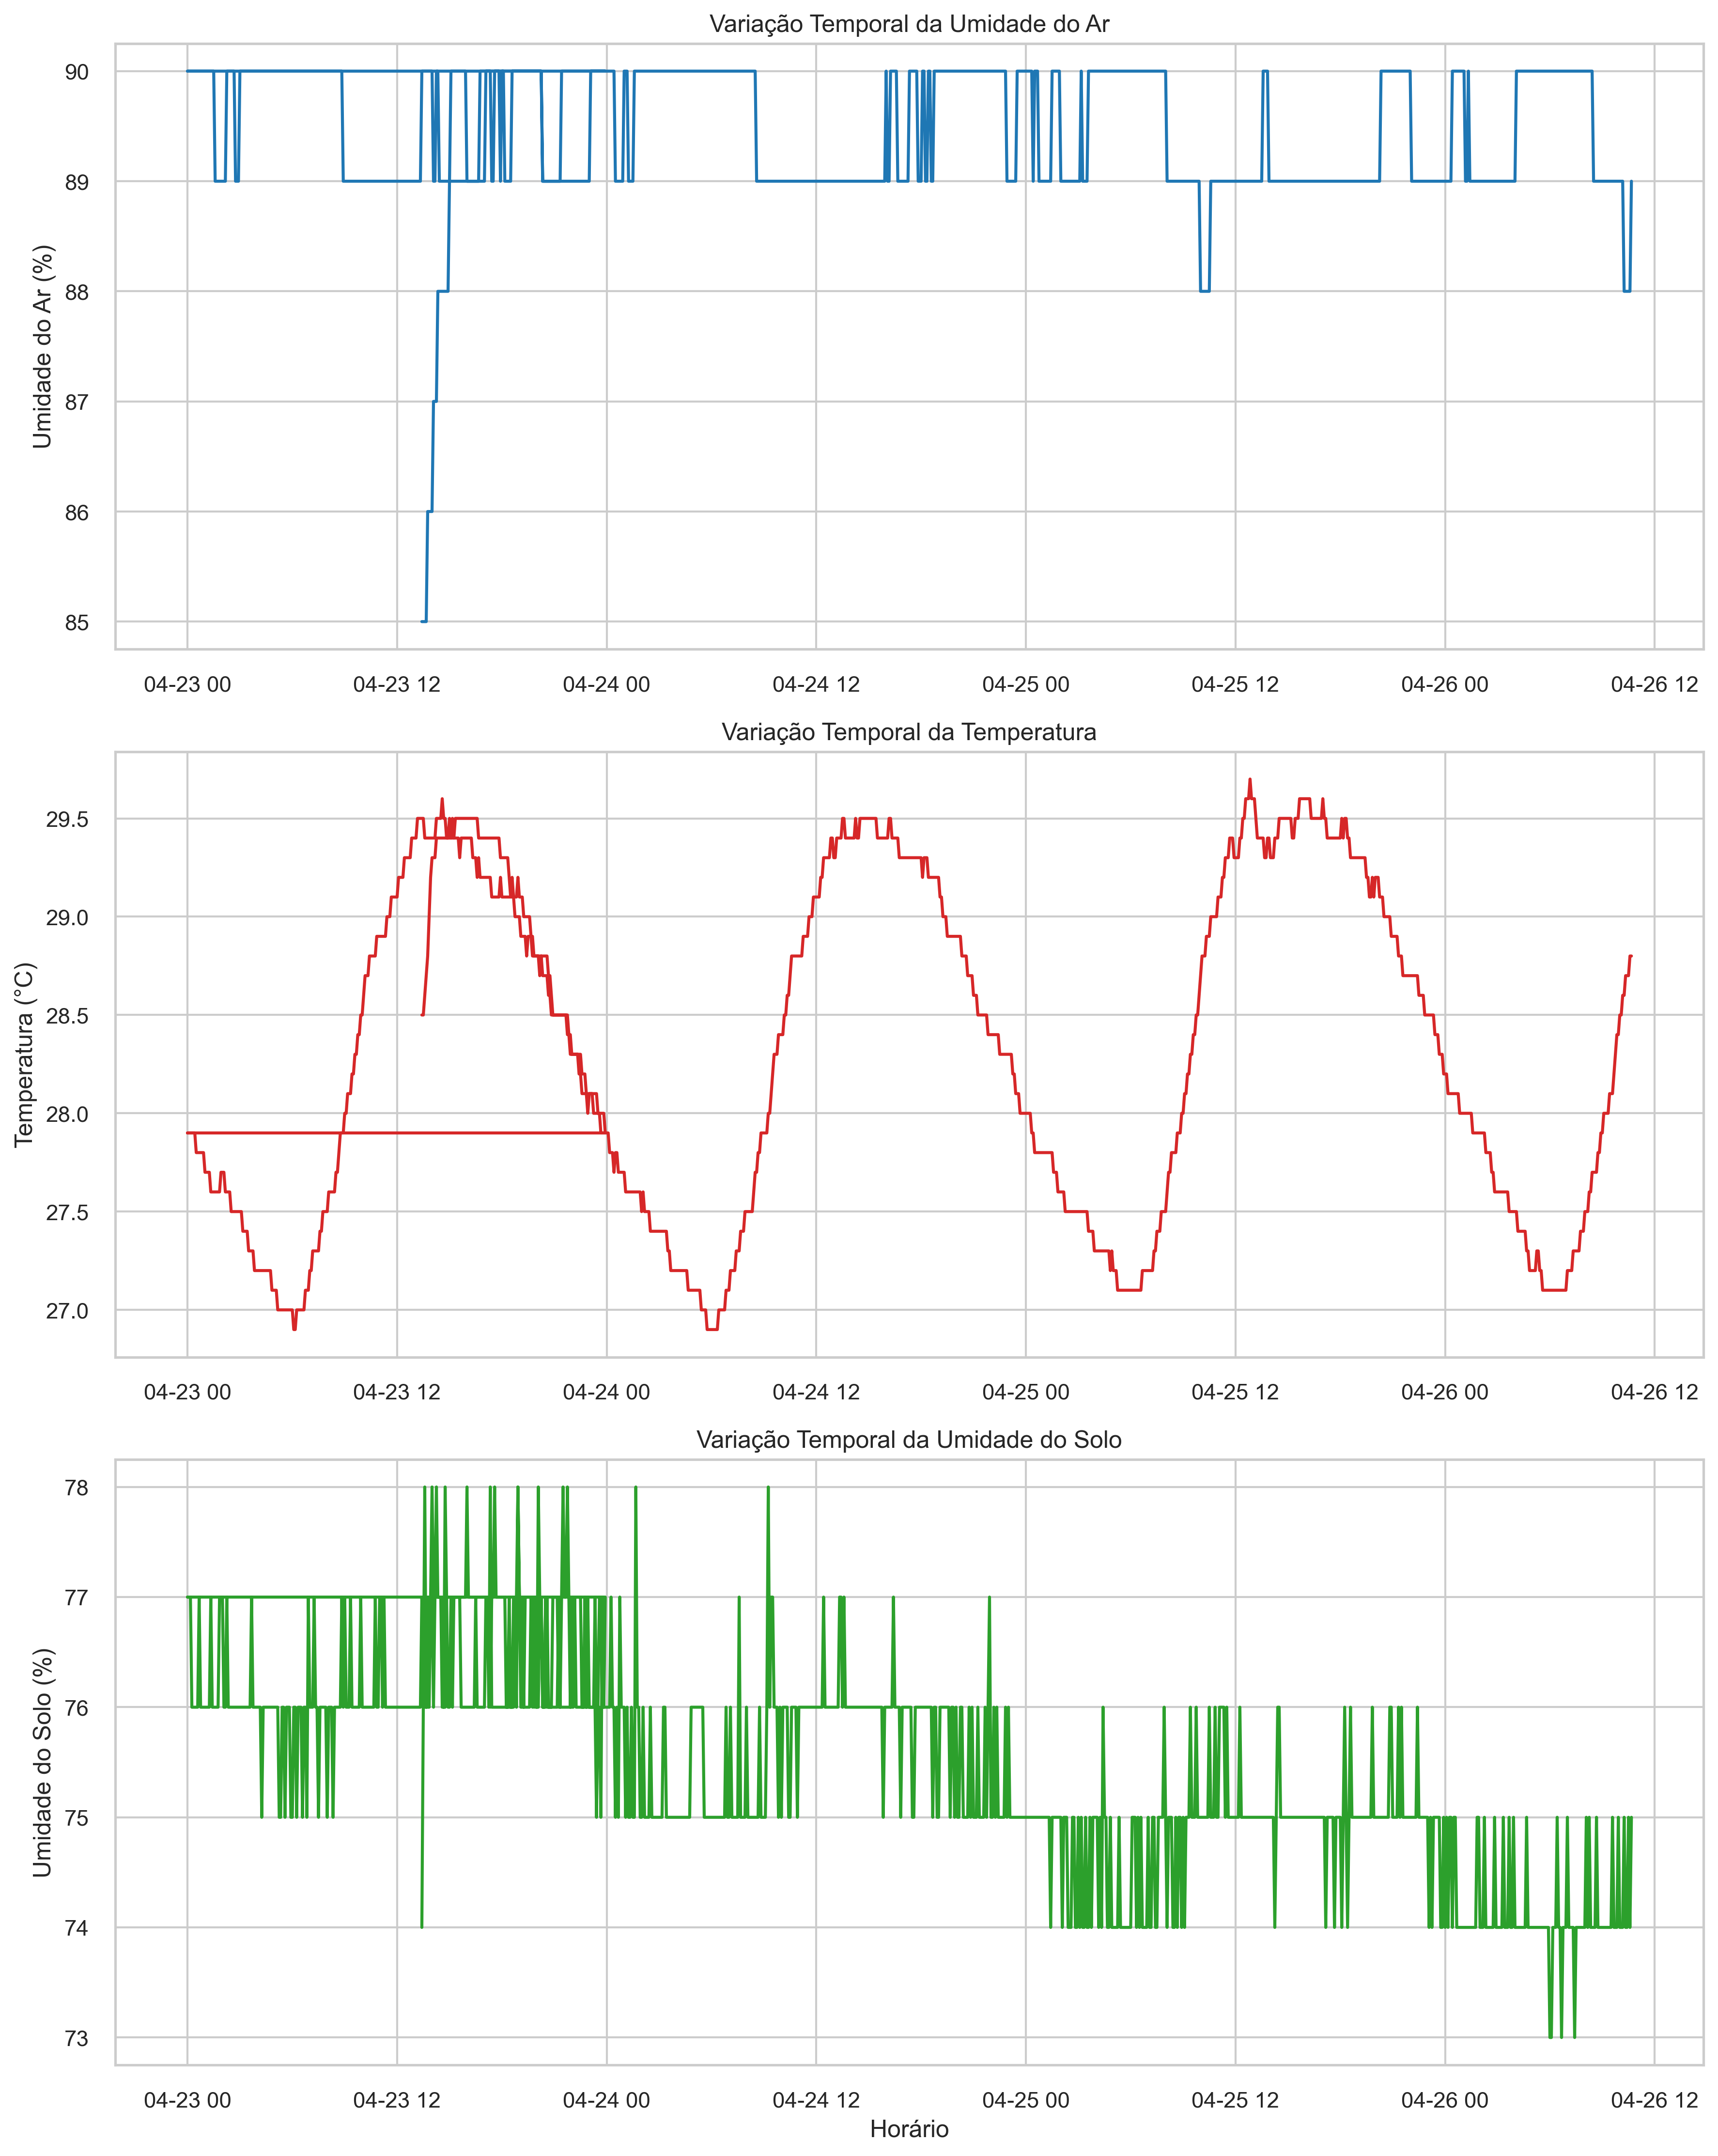
\includegraphics[width=0.9\textwidth]{graficos/temporal_combinado.png}
\caption{Variação temporal conjunta de umidade do ar, temperatura e umidade do solo.}
\label{fig:temporal_combinado}
\end{figure}

\subsection{Distribuição dos Dados}
\begin{figure}[H]
\centering
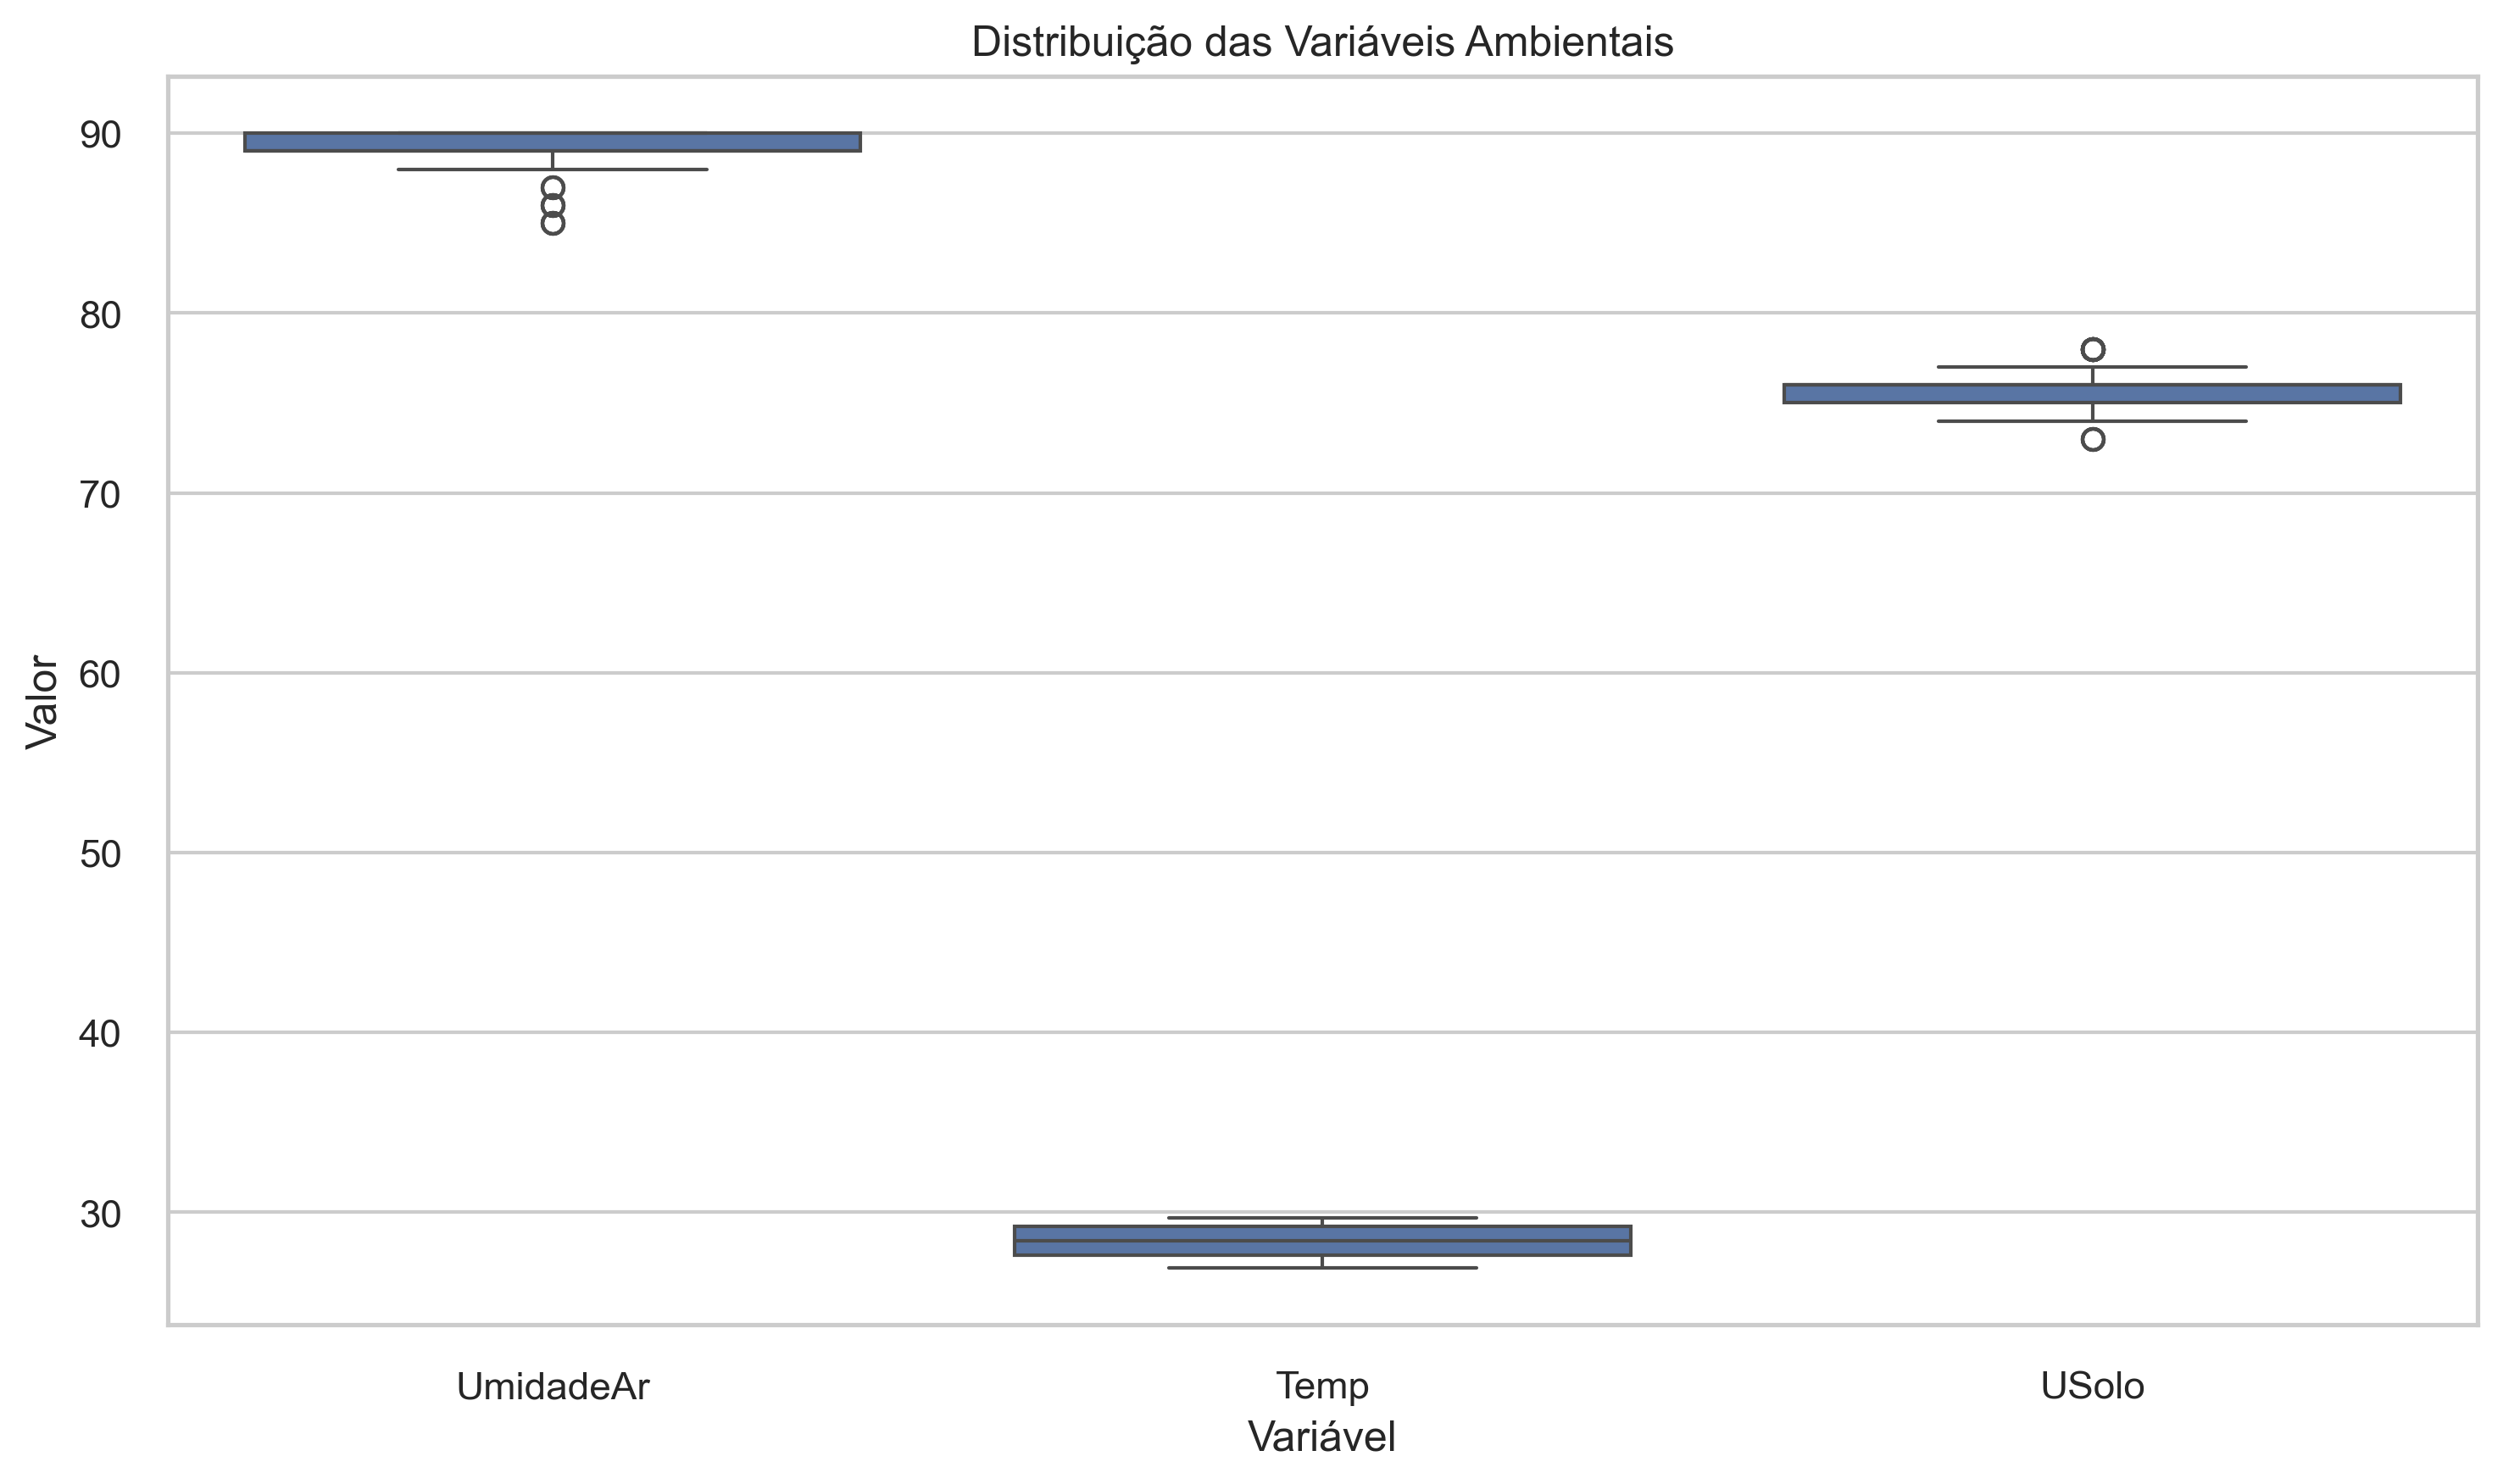
\includegraphics[width=0.9\textwidth]{graficos/boxplot_variaveis.png}
\caption{Distribuição estatística das variáveis ambientais}
\label{fig:boxplot}
\end{figure}

A Figura \ref{fig:boxplot} mostra a distribuição das variáveis, revelando:
\begin{itemize}
    \item Maior variabilidade na temperatura;
    \item Distribuição mais concentrada da umidade do solo;
    \item Leve assimetria nos dados de umidade do ar.
\end{itemize}

\subsection{Relações entre Variáveis}
\begin{figure}[H]
\centering
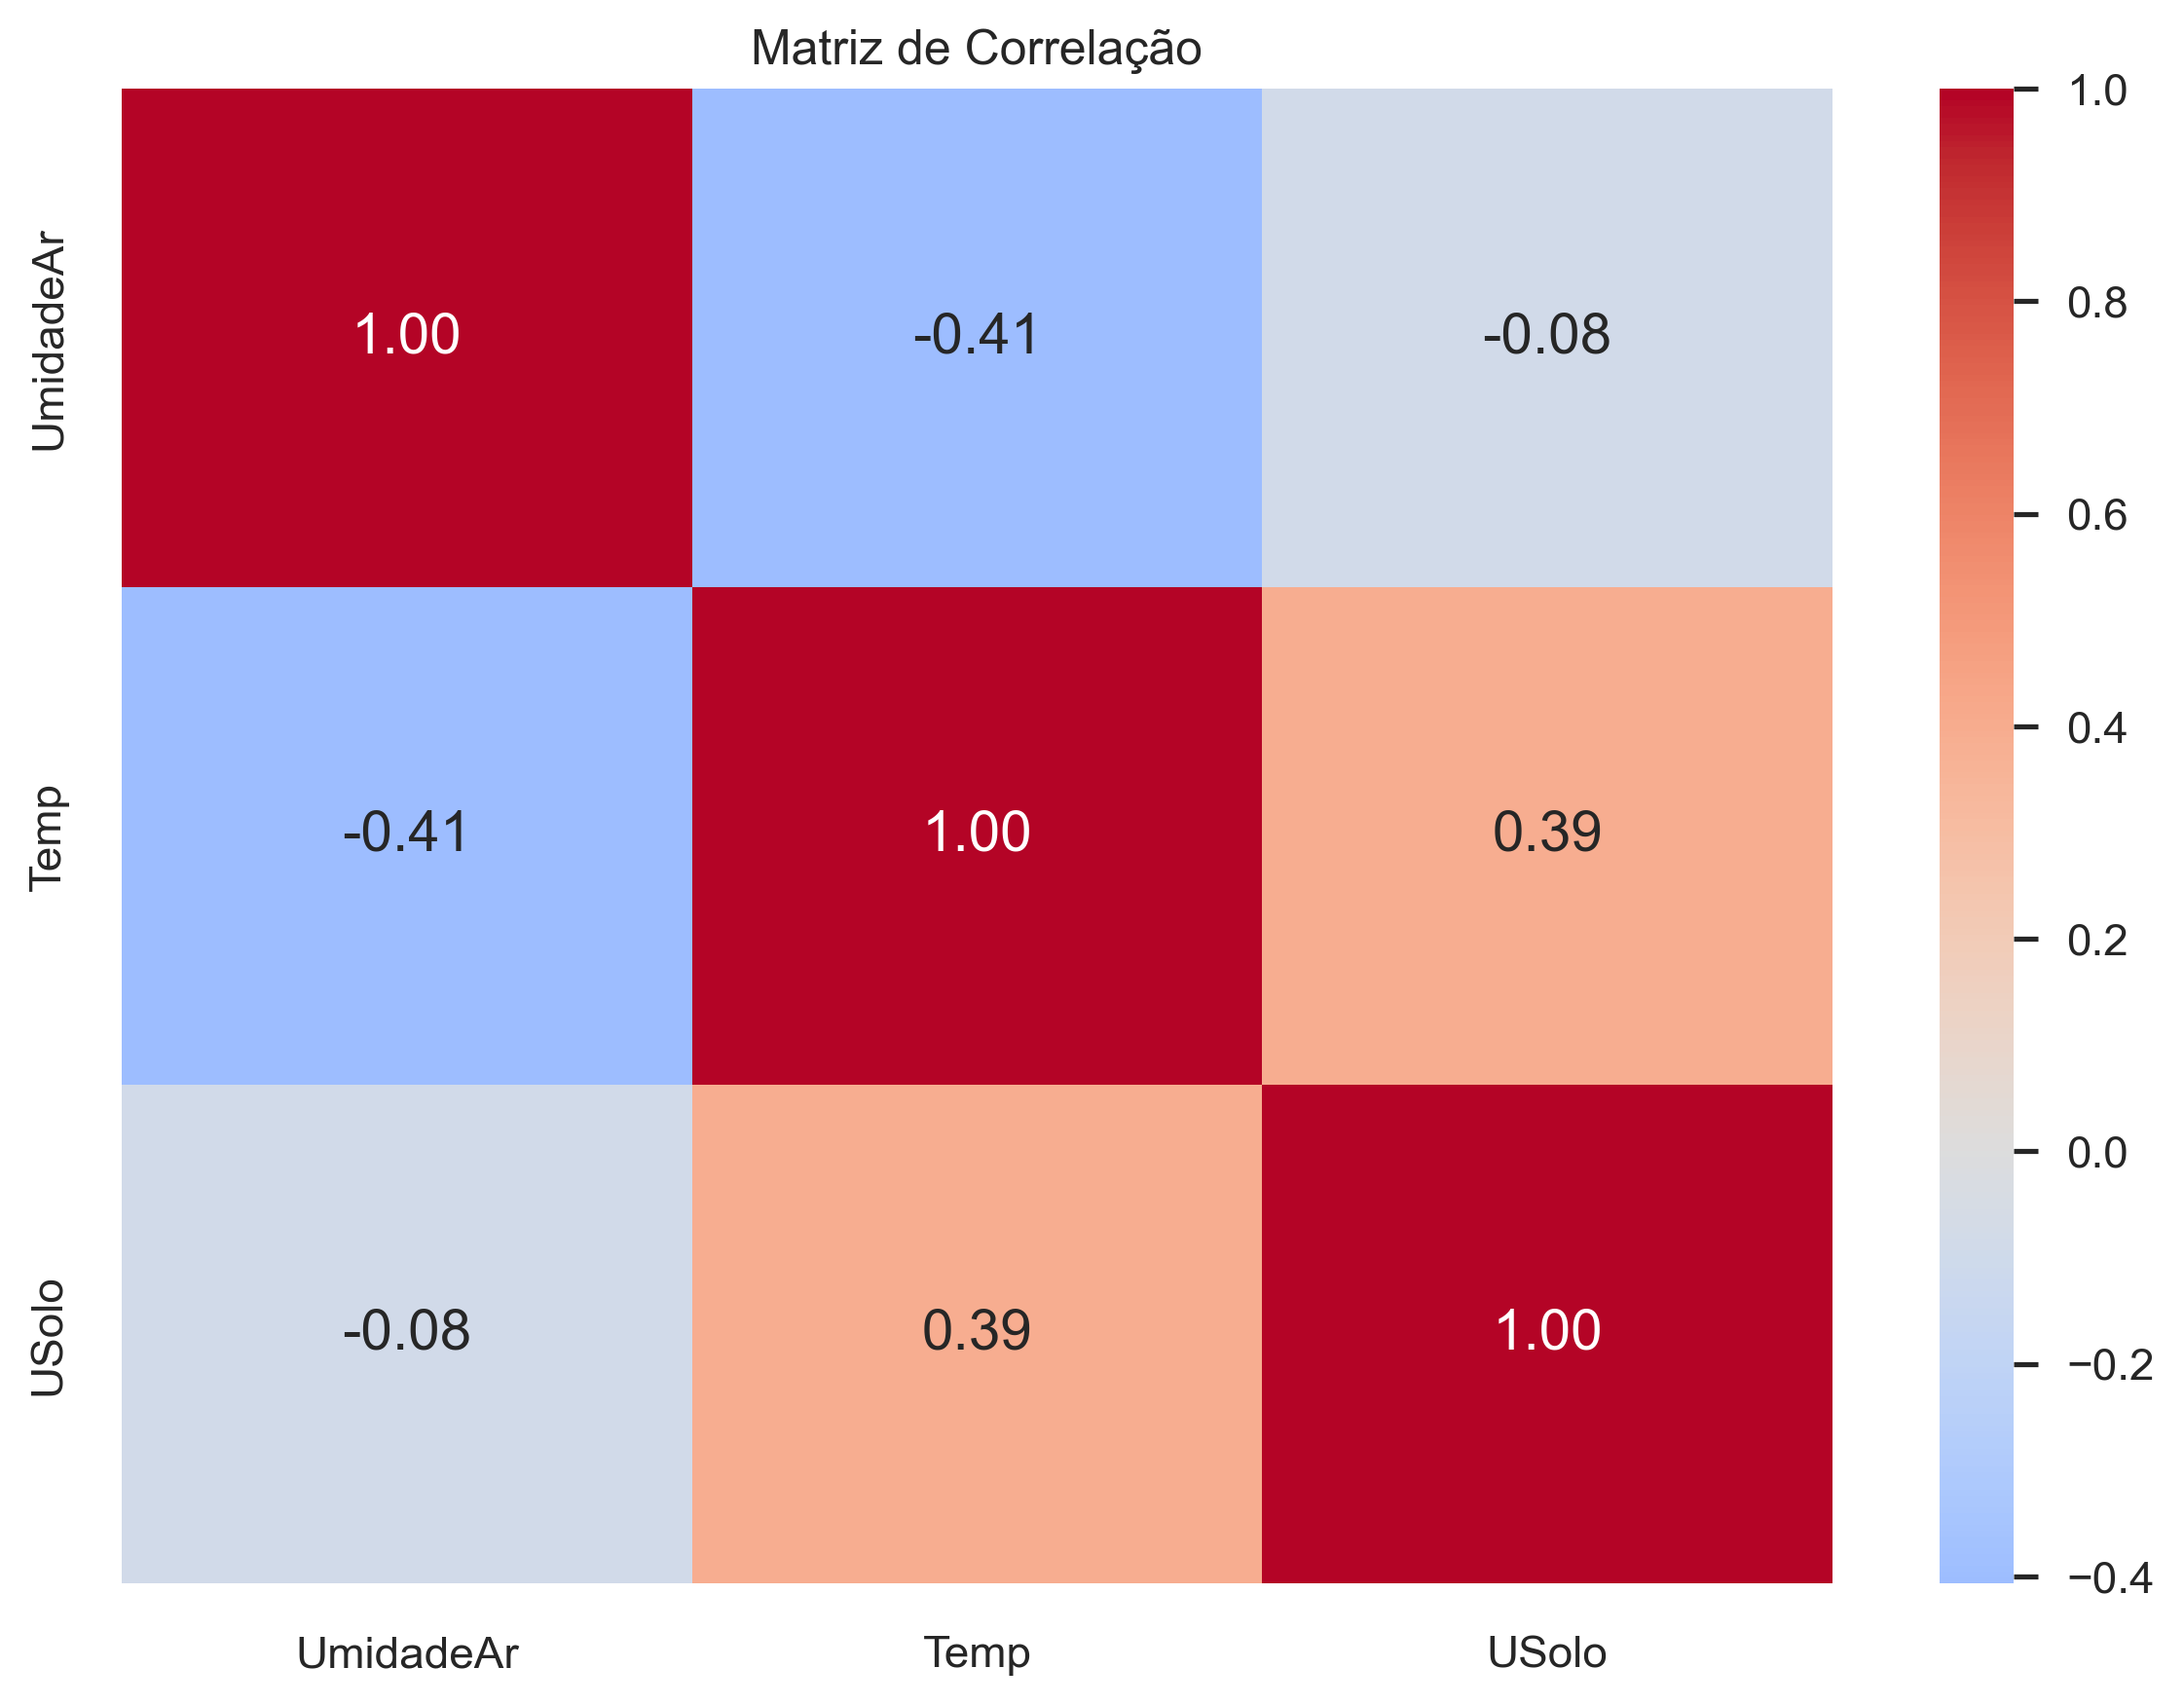
\includegraphics[width=0.8\textwidth]{graficos/matriz_correlacao.png}
\caption{Matriz de correlação entre as variáveis ambientais}
\label{fig:correlacao}
\end{figure}

A análise de correlação (Figura \ref{fig:correlacao}) destaca:
\begin{itemize}
    \item Correlação negativa moderada entre temperatura e umidade do ar (-0,41);
    \item Fraca relação entre umidade do solo e as demais variáveis.
\end{itemize}

\subsection{Análise de Outliers}
\begin{figure}[H]
\centering
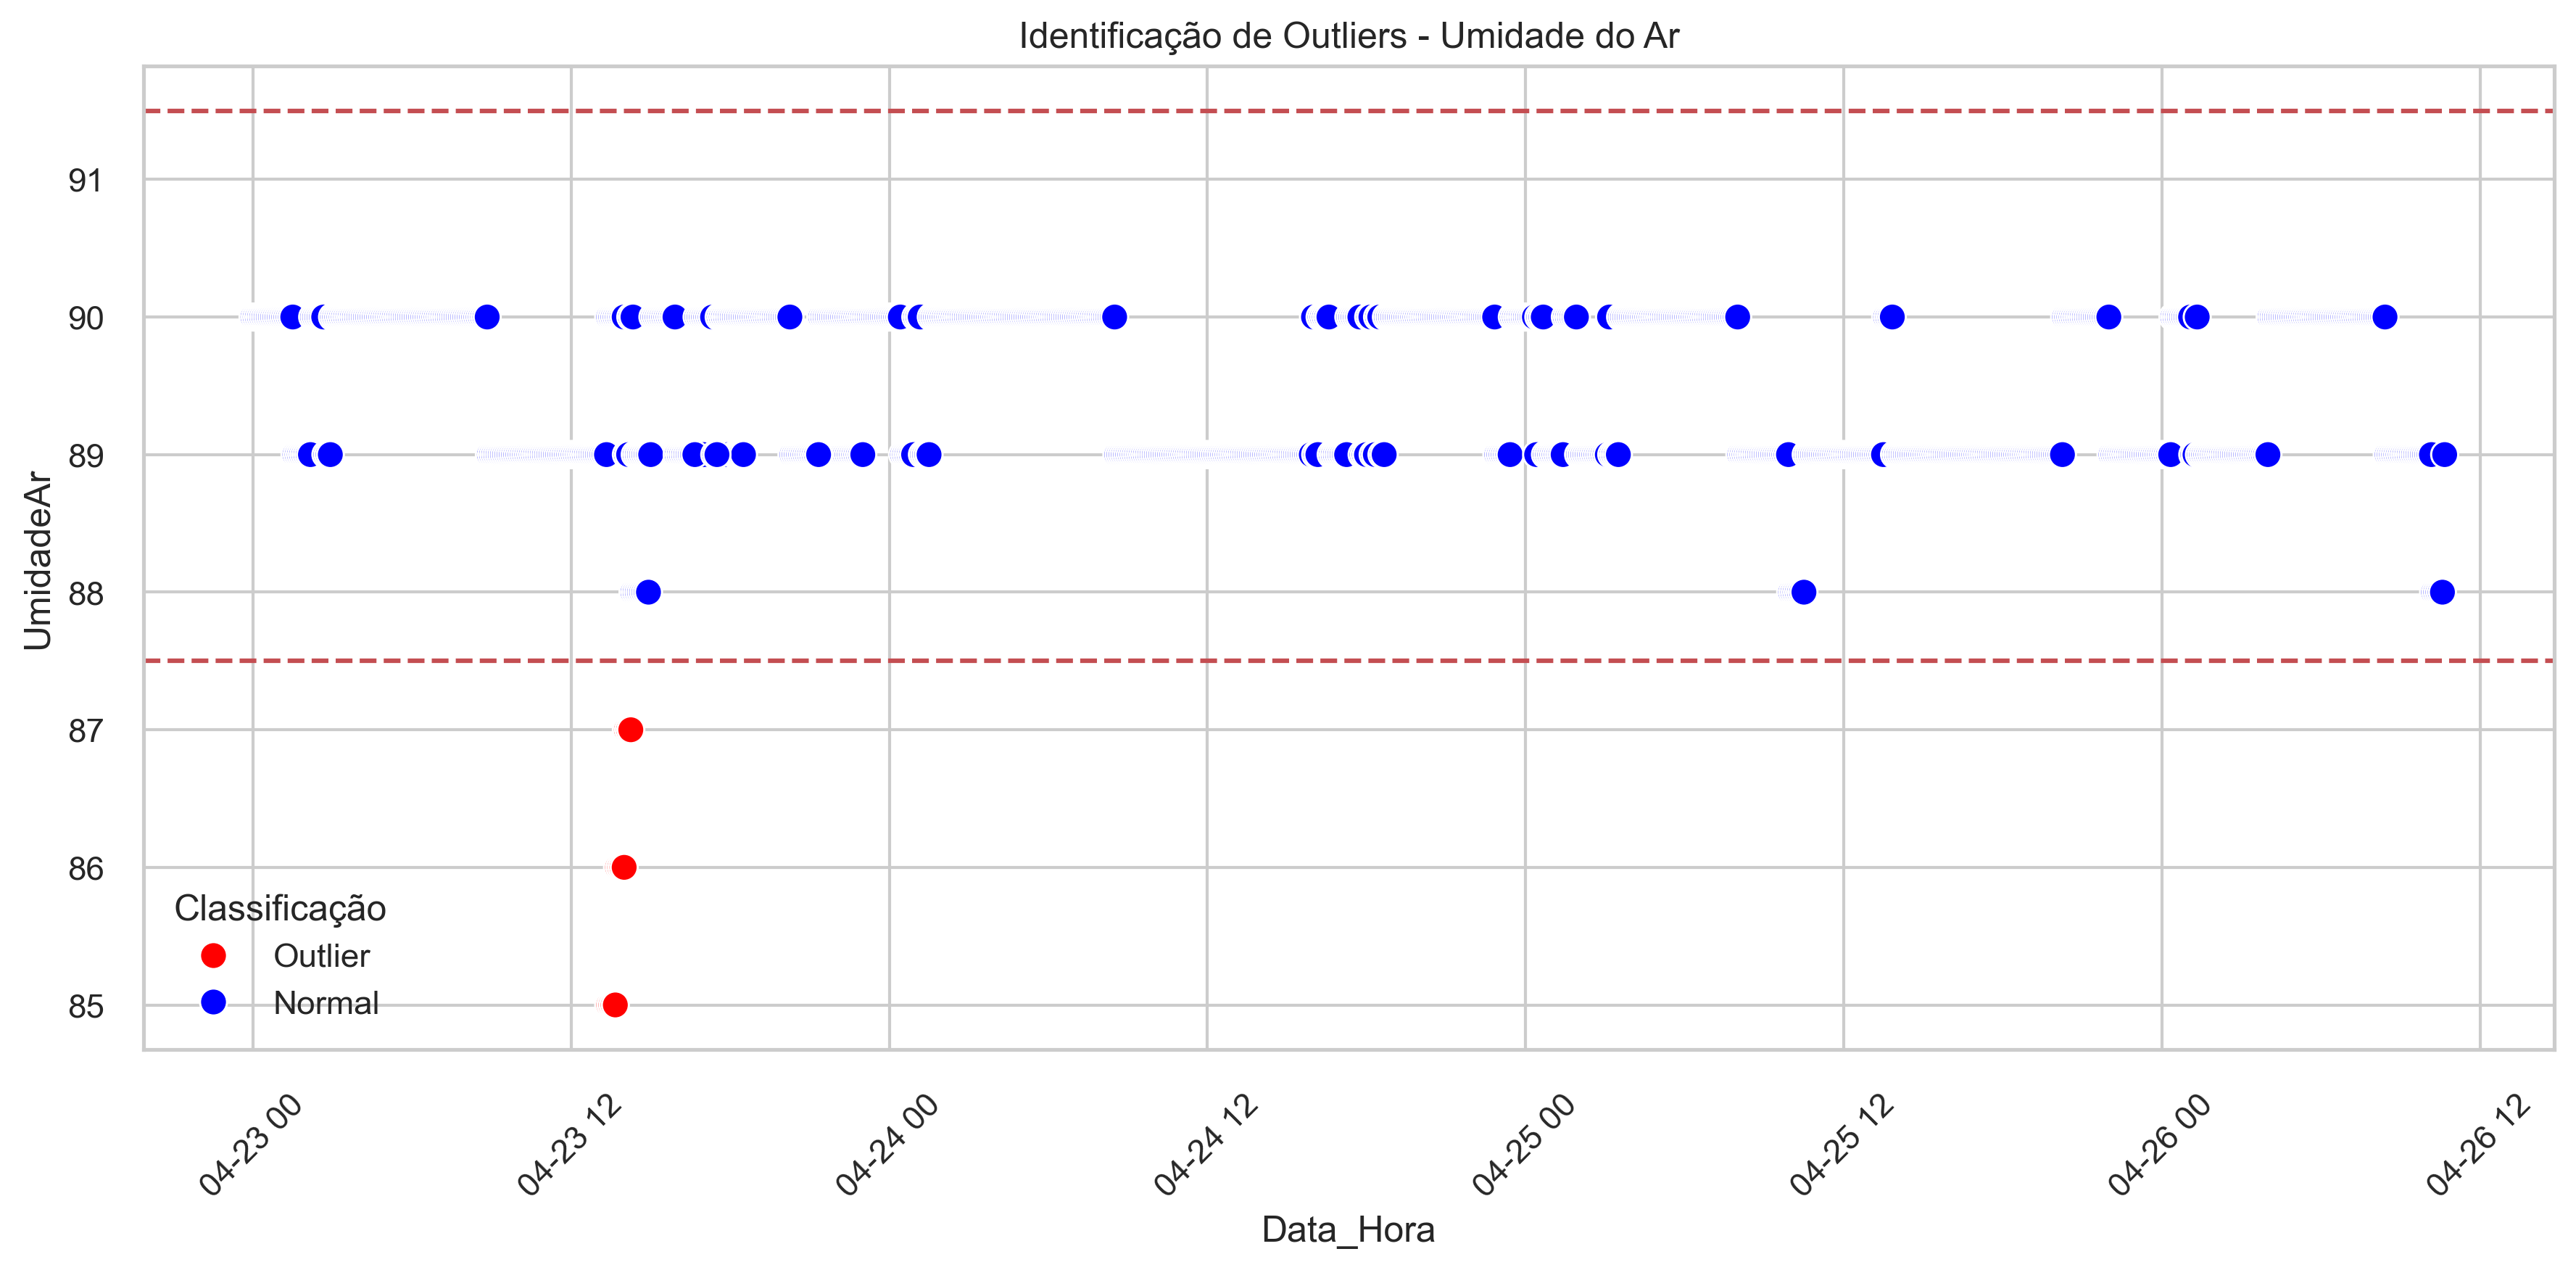
\includegraphics[width=0.8\textwidth]{graficos/outliers_umidade.png}
\caption{Identificação de outliers na umidade do ar}
\label{fig:outliers}
\end{figure}

A Figura \ref{fig:outliers} mostra os principais outliers detectados:
\begin{itemize}
    \item Leituras de 85\% em horários de aumento rápido da temperatura;
    \item Pequenas oscilações noturnas com variações de até 2\% da média.
\end{itemize}

\subsection{Análise Multivariada}
\begin{figure}[h]
\centering
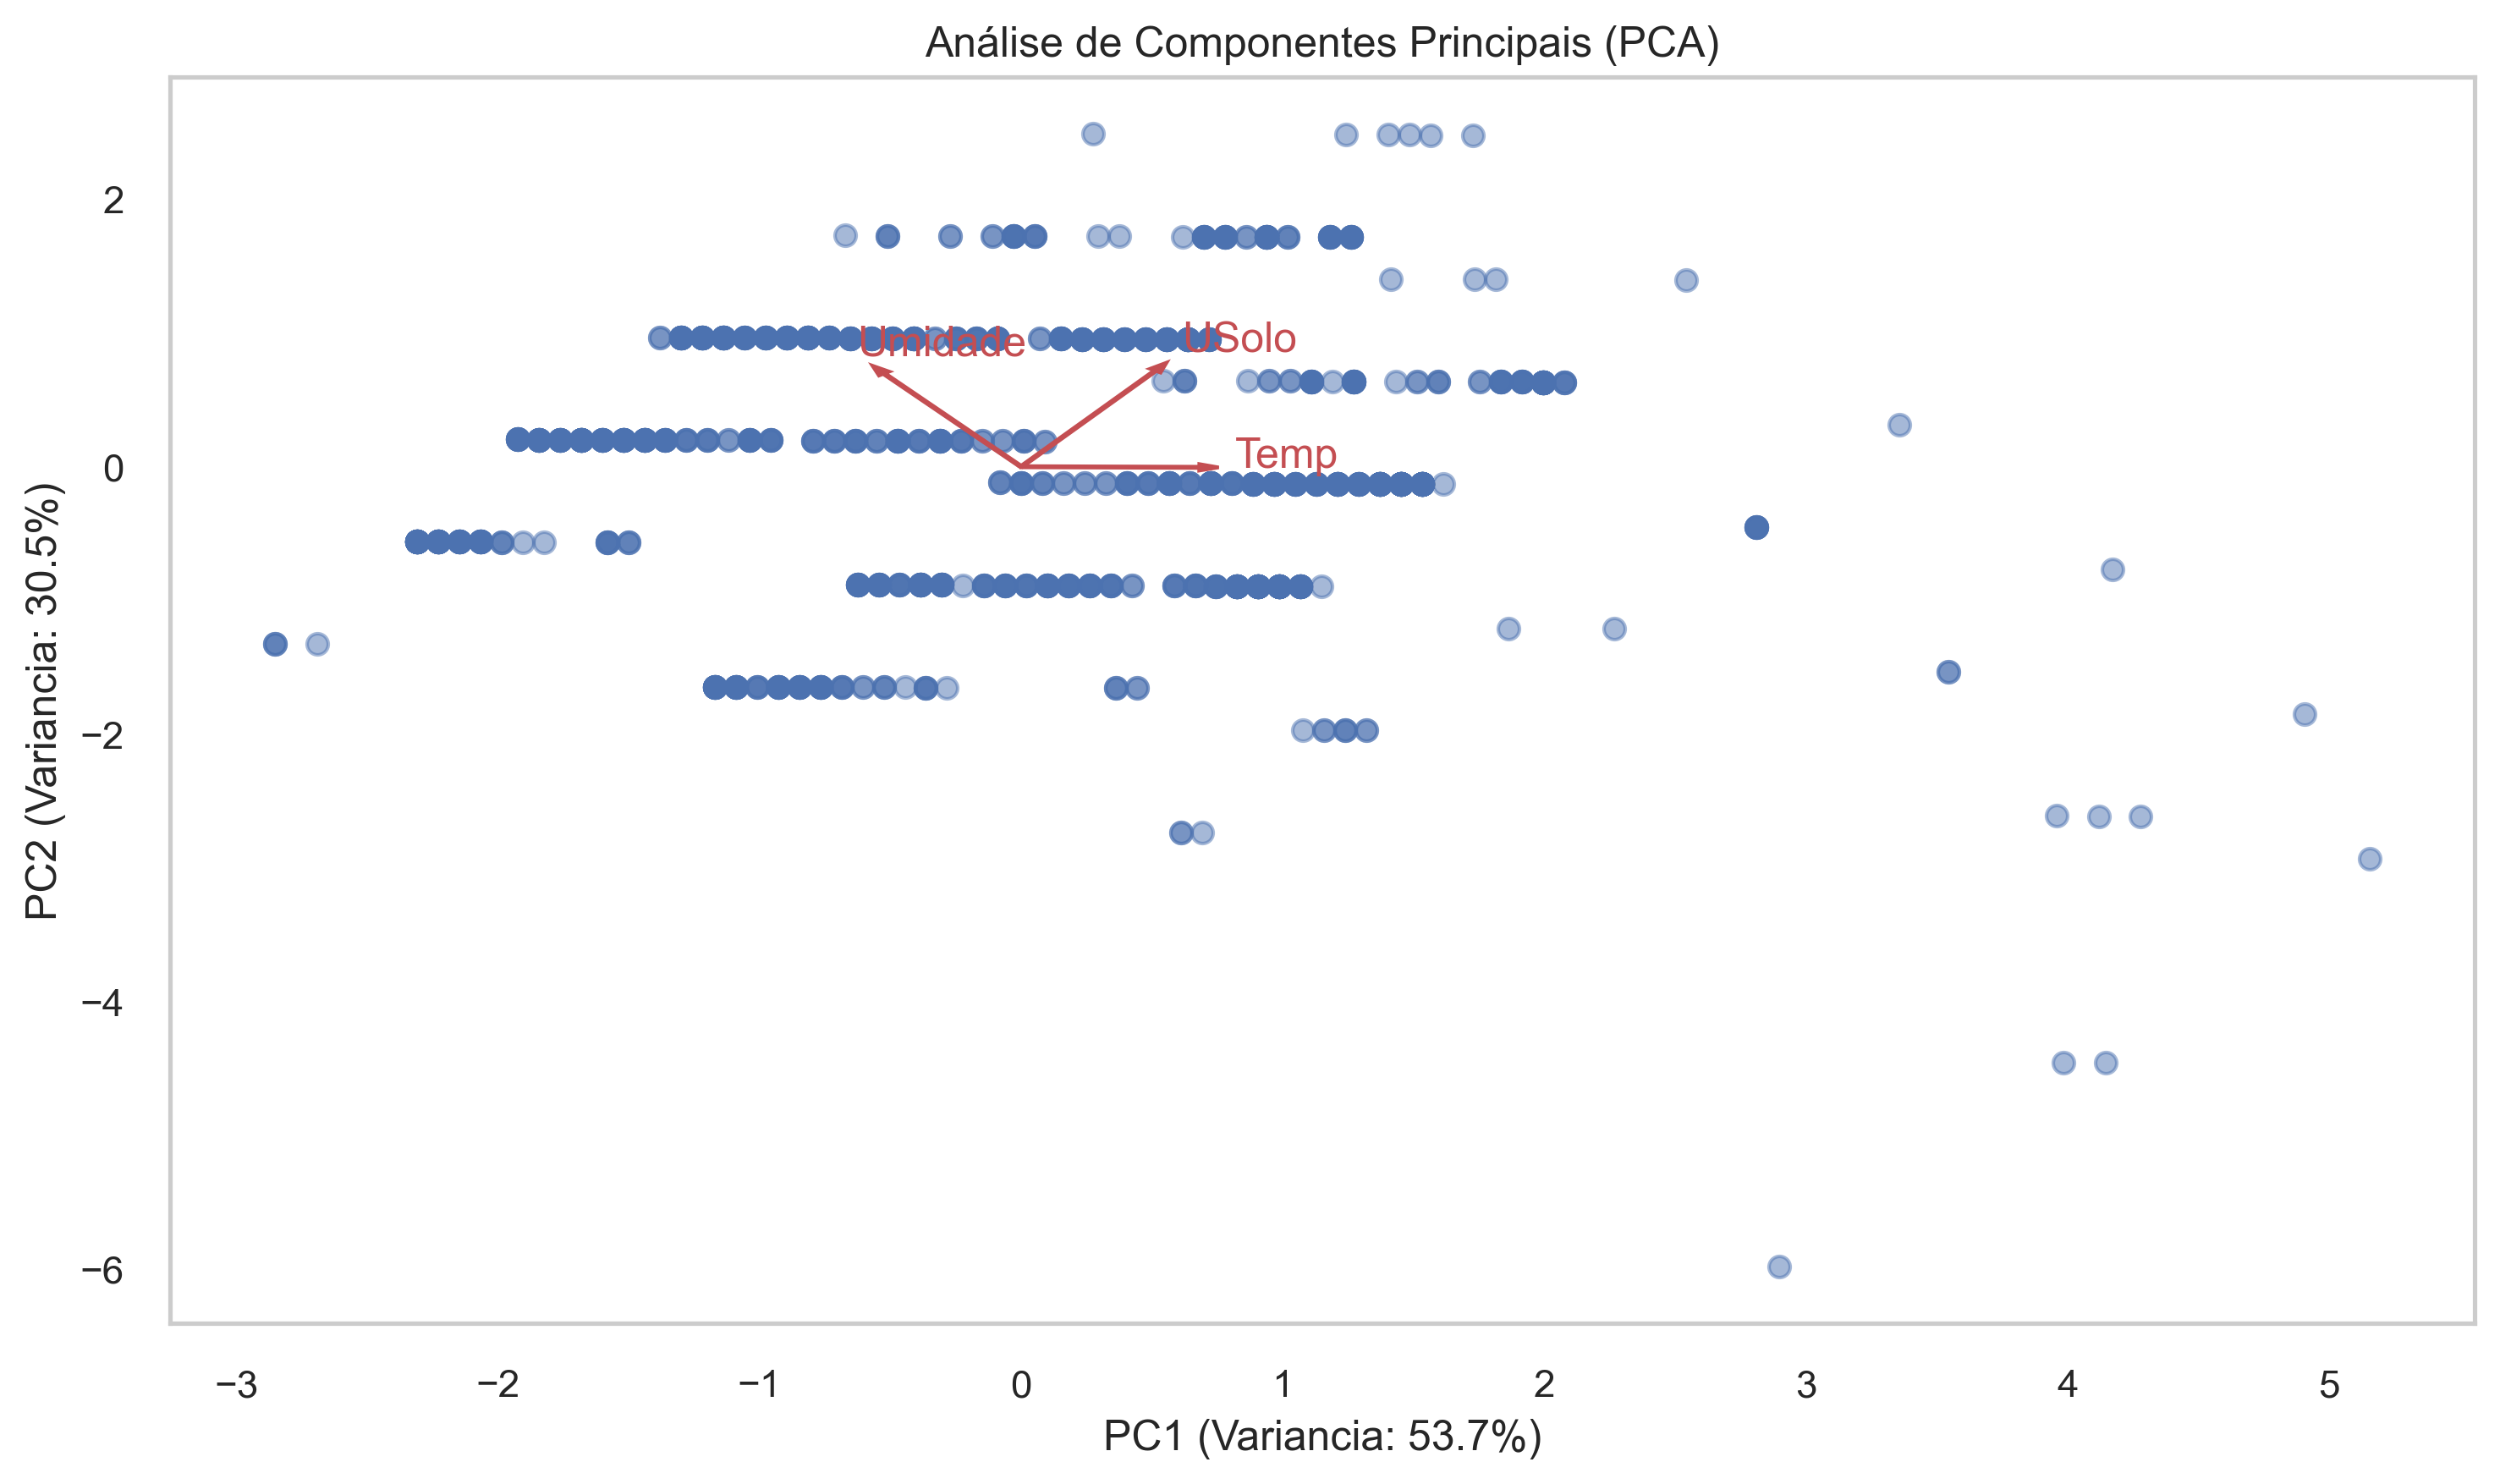
\includegraphics[width=0.8\textwidth]{graficos/pca_ambiental.png}
\caption{Análise de Componentes Principais das variáveis ambientais}
\label{fig:pca}
\end{figure}

A PCA (Figura \ref{fig:pca}) revela:
\begin{itemize}
    \item PC1 (64\% variância): principal contraste entre temperatura e umidade do ar;
    \item PC2 (28\% variância): relacionado à variabilidade da umidade do solo;
    \item Agrupamento consistente dos dados, com poucos desvios extremos.
\end{itemize}

Os resultados indicam:
\begin{itemize}
    \item Padrão circadiano nas variáveis ambientais (Figura \ref{fig:temporal_combinado});
    \item Relação inversa temperatura-umidade (Figura \ref{fig:correlacao});
    \item Estabilidade geral do sistema monitorado (Figura \ref{fig:boxplot});
    \item Estrutura multivariada organizada (Figura \ref{fig:pca}).
\end{itemize}


\subsection{Conclusão}
\label{sec:Conclusão}
A integração de Arduino com técnicas estatísticas mostrou-se viável, porém dependente de calibração e
poucos recursos de memória disponível. Conforme \cite{Tasiran2019}, a simplicidade do Arduino facilita prototipagem, mas limita
processamento de dados complexos. Soluções futuras podem incorporar edge computing, como proposto por \cite{Selmy2024},
para análise preditiva em tempo real. Além disso, a aplicação de redes neurais, discutida em \cite{MAHDAVINEJAD2018161},
poderia superar limitações de métodos tradicionais conjuntamente outra tecnológias para processamento mais complexo, por exemplo, uso em conjunto com Raspberry Pi. Nesse sentido, o trabalho demonstrou a viabilidade da integração de sensores com técnicas estatísticas para aplicações práticas. Os resultados indicam que a plataforma Arduino, combinada
com técnicas estátisticas, pode ser uma ferramenta poderosa para automação e monitoramento em tempo real.


Por fim, o artigo evidenciou que sensores de Arduino, combinados com técnicas estatísticas, são ferramentas
poderosas para análise de dados em IoT. Aplicações práticas em agricultura, saúde e indústria foram discutidas,
destacando-se a necessidade de calibração precisa e utilização de métodos estátisticos eficientes para uso em embarcados. Futuros trabalhos
devem explorar a integração com frameworks de deep learning e edge analytics, seguindo tendências apontadas por
\cite{Adi2020} e \cite{Selmy2024} e uso de atuadores e tecnologias como Raspberry Pi. \bibliographystyle{plain}
\bibliography{referencias}

\end{document}
